\documentclass[english]{scrartcl}

\usepackage{fullpage}
\usepackage{amstext,amssymb,amsmath,amsthm}
\usepackage{graphicx,subfigure}
\usepackage{multirow}
\usepackage{url}
\usepackage{hyperref}
\usepackage{color}

\graphicspath{{pics/}}

%\newtheorem{theorem}{Theorem}[section]
%\newtheorem{proposition}[theorem]{Proposition}


\title{Composite Bayesian inference}
\date{May 3, 2016}

\author{Alexis Roche\thanks{alexis.roche@\{centraliens.net,gmail.com,epfl.ch\}}}
%\\
%CHUV / Siemens Healthcare / EPFL \\ 
%CH-1015 Lausanne, Switzerland}

%\newcommand{\fix}{\marginpar{FIX}}
%\newcommand{\new}{\marginpar{NEW}}
%\newcommand{\matphi}{\boldsymbol{\Phi}} 
%\def\x{{\mathbf{x}}}
%\def\z{{\mathbf{z}}}
%\def\u{{\mathbf{u}}}
%\def\p{{\bar{\mathbf{p}}}}
%\def\q{{\bar{\mathbf{q}}}}



\begin{document}

\maketitle

\begin{abstract}
This paper revisits the concept of composite likelihood from the perspective of probabilistic inference, and proposes a generalization called {\em super composite likelihood} for sharper inference in multiclass problems. It is argued that, beside providing a new interpretation and a general justification of na\"ive Bayes procedures, super composite likelihood yields a much wider class of discriminative models suitable for unsupervised and weakly supervised learning.
\end{abstract}


\section{Introduction}
\label{sec:intro}

Conventional Bayesian inference and other likelihood-based paradigms rest upon the existence of a statistical data-generating model that is both experimentally plausible and computationally tractable. Because this is challenging when the data is inherently complex, common practice to implement feasible inference algorithms is to use deliberately misspecified data-generating models \cite{White-82,Walker-13} such as in {\em na\"ive Bayes} \cite{Ng-01} or minimum description length \cite{Grunwald-07}, or to resort to highly supervised discriminative modeling approaches \cite{Ng-01}, not to mention ad-hoc methodology.

Composite likelihood (see \cite{Varin-11} and the references therein) is a middle-way approach that extends the familiar notion of likelihood without requiring a full data-generating model. The key idea is to model an arbitrary set of low-dimensional features separately and then combine them, instead of modeling the data distribution as a whole. This may also be viewed as a {\em divide \& conquer} method of approximating the actual likelihood. While maximum composite likelihood does not inherit the general property of maximum likelihood to yield asymptotically minimum-variance estimators, it may offer an excellent trade-off between computational and statistical efficiency. 

In this note, composite likelihood is interpreted as a probabilistic opinion pool \cite{Genest-86,Garg-04} of ``agents'' using different pieces of information, or clues, extracted from the data. Each agent acts as a local Bayesian statistician expressing an opinion in the form of a posterior distribution on the unknown parameters of interest, or hypotheses, given a specific clue. Composite likelihood can therefore be associated with a probability distribution on hypotheses, hence extending Bayesian analysis to problems where the proper likelihood function is intractable.

I further justify a generalization of composite likelihood called {\em super composite likelihood} whereby clues can be weighted differently depending on hypotheses to better deal with multiclass inference problems. This more general concept also encompasses another likelihood approximation strategy known as {\em PDF~projection} \cite{Baggenstoss-03,Minka-04,Baggenstoss-15}.

This paper is intended to serve as supporting material for a companion paper (in preparation), where the super composite likelihood framework is applied in computer vision to develop a probabilistic theory of image registration \cite{Viola-97}.


\section{Composite likelihood as opinion pooling}
\label{sec:pool}

Let $Y$ an observable multivariate random variable with sampling distribution $p(y|\theta)$ conditional on some unobserved parameter of interest, $\theta\in\Theta$, where $\Theta$ is a known set. Given an experimental outcome $y$, the likelihood is the sampling distribution evaluated at $y$, seen as a function of $\theta$:
$$
L(\theta) = p(y|\theta)
.
$$

For a high-dimensional $Y$, this expression may be intractable if a plausible generative model is lacking, or involves nuisance parameters that are cumbersome to integrate out. A natural workaround known as {\em data reduction} is then to extract some lower-dimensional feature $z=f(y)$, where $f$ is a many-to-one mapping, and consider the potentially more convenient likelihood function:
$$
\ell(\theta) = p(z|\theta)
.
$$

Substituting $L(\theta)$ with $\ell(\theta)$ boils down to restricting the sample space, thereby  ``delegating'' statistical inference to an ``agent'' provided with partial information. While it is valid for such an agent observing~$z$ only to consider $\ell(\theta)$ as the likelihood function of the problem, the drawback is that $\ell(\theta)$ might be poorly informative about~$\theta$ due to the information loss incurred by data reduction. To make the trick statistically more efficient, we may extract several features, $z_i=f_i(y)$ for $i=1,2,\ldots,n$, and try to aggregate the likelihood functions $\ell_i(\theta) = p(z_i|\theta)$ that they elicit.

This leads to a classical problem of combining probabilistic opinions from possibly redundant agents \cite{Tarantola-82,Genest-86,Garg-04,Allard-12}. Genest {\em et al} \cite{Genest-86b} showed, in particular, that the only pooling operator that does not explicitly depend on~$\theta$ and preserves {\em external Bayesianity} is the generalized logarithmic opinion pool:
\begin{equation}
\label{eq:log_pool}
p_\star(\theta) = \frac{1}{Z} \pi(\theta) \prod_{i=1}^n \ell_i (\theta)^{w_i},
\qquad
{\rm with}\quad 
Z = \int \pi(\theta) \prod_{i=1}^n \ell_i (\theta)^{w_i} d\theta,
\end{equation} 
where $\pi(\theta)$ is some reference distribution or prior, and $w_i$ are arbitrary positive\footnote{Negative weights can be chosen only if the parameter set $\Theta$ is finite \cite{Genest-86b}.} weights that sum up to one,
$$
\sum_{i=1}^n w_i = 1
.
$$

External Bayesianity essentially means that it should not matter whether a prior on~$\theta$ is incorporated before or after pooling opinions, provided that all agents agree on the same prior. Importantly, the log-linear pool does not assume mutual feature independence, as would the same factorized form as (\ref{eq:log_pool}) with all unitary weights, $w_1=\ldots=w_n= 1$. Instead, redundancy between agents is assumed by default, and is effectively encoded by the unit sum constraint on weights\footnote{Nevertheless, features which are {\em known} to be mutually independent can be merged into a single feature. This results in increasing their weights in the log-linear pool.}.

Strikingly, (\ref{eq:log_pool}) reduces to an analogous of Bayes rule: $p_\star(\theta)\propto \pi(\theta) L_c(\theta,\mathbf{w})$, where $\mathbf{w}=(w_1,w_2,\ldots,w_n)^\top$ denotes the vector of weights, and the quantity:
\begin{equation}
\label{eq:comp_lik}
L_c(\theta,\mathbf{w}) \equiv \prod_{i=1}^n \ell_i (\theta)^{w_i}
\end{equation} 
plays exactly the same role as a traditional likelihood function. $L_c(\theta,\mathbf{w})$ shares a convenient factorized form with the likelihood derived under mutual feature independence, sometimes called {\em na\"ive Bayes} likelihood in the literature \cite{Ng-01}. The key difference is that the single-feature likelihoods are scaled by positive weights~$w_i$ smaller than one, hence producing a flatter posterior distribution. In comparison with the proper likelihood (not assuming feature independence), the clear computational advantage is that we only need to evaluate the marginal feature distributions, rather than the joint distribution of all features. 

We recognize in~(\ref{eq:comp_lik}) a general expression known as a {\em marginal composite likelihood} \cite{Varin-11}, although it is derived here under the restriction that the weights sum up to one (as already motivated in \cite{Wang-14} by a different argument using the maximum entropy principle). 
% Accounting here for Xi'An comment on xianblog.wordpress.com
% The sum of the powers is constrained to be equal to one, even though
% I do not understand why the dimensions of the projections play no
% role in this constraint. Simplicity is advanced as an argument,
% which sounds rather weak…
This simple constraint is implied by the external Bayesianity requirement: as it turns out, the only aggregation operator which is both externally Bayesian and independent from $\theta$ boils down to plugging a composite likelihood with unit sum weights into Bayes rule, hence extending the classical notion of likelihood in Bayesian analysis.

Previous attempts at Bayesian composite likelihood include tuning a constant weight so as to best adjust the pseudo posterior variance matrix to the asymptotic variance matrix of the maximum composite likelihood estimator \cite{Pauli-11}, or performing a close-in-spirit curvature adjustment \cite{Ribatet-12}. Such approaches reconcile the frequentist and Bayesian notions of uncertainty to some extent, but are not externally Bayesian since they do not warrant unit sum weights. When we refer to composite likelihood in the sequel, we assume unit sum weights.

%It is an open problem to determine weights that make it appropriate to plug composite likelihood into Bayes rule. The recommendation for unit sum weights is particularly simple compared to, {\em e.g.}, tuning a constant weight so as to best adjust the pseudo posterior variance matrix to the asymptotic variance matrix of the maximum composite likelihood estimator \cite{Pauli-11}, or performing a close-in-spirit curvature adjustment \cite{Ribatet-12}. Such approaches reconcile the frequentist and Bayesian notions of uncertainty to some extent, but are not externally Bayesian since they do not warrant unit sum weights. When we refer to composite likelihood in the sequel, we assume unit sum weights.


\section{Composite likelihood as message approximation}
\label{sec:message}

Composite likelihood may also be understood as a means to approximate the ``true'' likelihood function\footnote{By {\em true likelihood}, we mean the likelihood corresponding to a specified yet intractable generative model. In practice, such a model is obviously not required.} or, in the language of graphical models, the {\em message} that the data sends to the latent variable~$\theta$. Several ``clues'' are sent to~$\theta$ via different data features, and then integrated assuming {\em non-coalescent} emitting sources, meaning that statistical dependences between clues are treated as unknown, although not ignored. The whole idea is depicted by the factor graph\footnote{See \cite{Bishop-06} for a didactic introduction to factor graphs.} in Figure~\ref{fig:fgraph2}, where the latent variable is connected to multiple factors involving single clues (rather than a single factor involving multiple clues), thereby enabling efficient computations.

%A simplified message is computed by extracting arbitrary features from the data and treating them as {\em non-coalescent} clues in the sense that their statistical dependences are not modeled (although not ignored). 

\begin{figure}[!ht]
\begin{center}
\subfigure[Generative model]{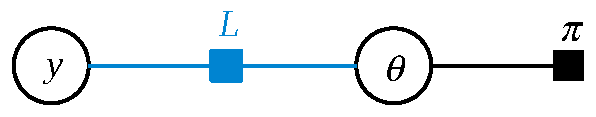
\includegraphics[width=.35\textwidth]{fgraph1.pdf}\label{fig:fgraph1}}
\subfigure[Composite likelihood model]{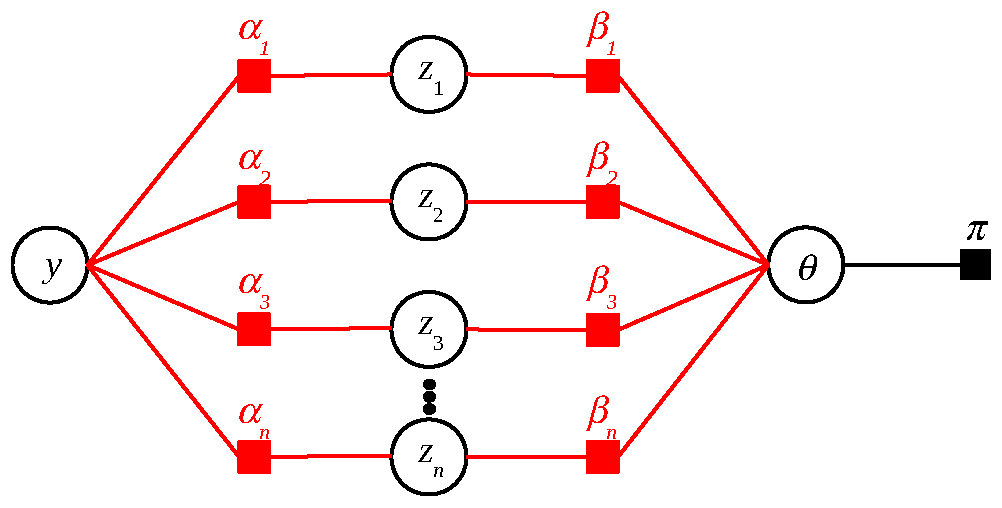
\includegraphics[width=.6\textwidth]{fgraph2.pdf}\label{fig:fgraph2}}
\caption{Factor graph representations of a generative model (a) and its approximation using composite likelihood (b). In (a), the factor connecting the data~$y$ and the latent variable~$\theta$ is the true likelihood, $L(y,\theta)=p(y|\theta)$. In (b), factors connecting~$y$ and the clues $z_1,z_2,\ldots$ represent feature extractions, $\alpha_i(y,z_i)=\delta[z_i-f_i(y)]$, while factors connecting the clues and~$\theta$ are scaled single-feature likelihoods, $\beta_i(z_i,\theta)=p(z_i|\theta)^{w_i}$. In both graphs, the factor shown in black is the prior $\pi(\theta)$.}
\label{fig:fgraph}
\end{center}
\end{figure}

This approximation scheme happens to be optimal in an information-theoretic sense. As noted in \cite{Garg-04}, the log-linear pool minimizes the average Kullback-Leibler (KL) divergence to the probabilistic opinions:
\begin{equation}
\label{eq:avg_kl}
p_\star = \arg\min_p \sum_{i=1}^n w_i D(p\|p_i),
\end{equation}
where $p_i(\theta) \propto \pi(\theta)\ell_i(\theta)$ is the posterior distribution of agent~$i$. Note that, even though the weights are arbitrary in~(\ref{eq:avg_kl}), the optimal solution normalizes them to unit sum. Composite likelihood thus arises as the best possible consensus among agents according to a natural criterion, in addition to satisfying the external Bayesianity axiom. 

If one interprets the average divergence from agent opinions~(\ref{eq:avg_kl}) as a proxy for the divergence from ``the truth'', $p(\theta|y)$, composite likelihood can be seen as a variational approximation to the true likelihood. This corresponds to the intuitive notion that a consensus among sufficiently many experts should yield a reasonable guess. An essential difference with usual approximate inference methods \cite{Bishop-06,Minka-05} is that the likelihood function does not need to be computable owing to the use of a proxy. However, as we shall see in Section~\ref{sec:weights}, knowledge of the feature sampling distributions can be further exploited to optimize the likelihood approximation with respect to the composite likelihood weights.


\section{Super composite likelihood}
\label{sec:super}

Due to the distribution of weights between clues, a drawback of composite likelihood is that it is prone to {\em information overload} in the sense that it tends to ``flatten out'' when too many clues are included as relevant clues then get downweighted. If one decides not to merge clues for computational reasons (this would require handling their joint distribution), one could hope to mitigate information overload by assigning strong weights only to those clues that are believed to be ``most informative''. 

However, when chosen for computational simplicity, clues may not only convey limited information at individual level: their informativeness may also be very much hypothesis-dependent. Consider, for instance, diagnosing a disease from a routine medical checkup. Body temperature may point to a bacterial infection by comparison with normality, but would not help detecting a non-infectious cardiovascular disease -- and conversely for, say, blood pressure.

This motivates a more general setting where clues can be weighted differently depending on hypotheses. To avoid unnecessary technicalities, we will assume from now on a finite set of hypotheses, $\Theta=\{\theta_0,\theta_1,\ldots,\theta_m\}$, where one particular hypothesis, $\theta_0$, is given the special status of reference, or ``null'' hypothesis. 

We start by introducing auxiliary binary variables~$t_j$, for $j=1,\ldots,m$, defined by truncation of~$\theta$:
\begin{equation}
\label{eq:binary}
t_j = 
\left\{
\begin{array}{lll}
1 & {\rm if} & \theta = \theta_j \\
0 & {\rm if} & \theta = \theta_0
\end{array}
\right.
.
\end{equation}
One can think of each~$t_j$ as an indicator light that flashes green or red whenever~$\theta$ is in one of the particular two states $\theta_j$ or $\theta_0$, and does not respond otherwise. The collection of all $t_j$'s may be thought of as a population code \cite{Knill-04} for~$\theta$. 

The key idea is as follows: instead of approximating the message sent from the data to~$\theta$ in one piece as in Section~\ref{sec:message}, we may approximate each of the simpler messages sent to the $t_j$'s. To that end, we construct a factor graph using the population code, depicted in Figure~\ref{fig:fgraph3}, which is equivalent to the graph in Figure~\ref{fig:fgraph1} for the purpose of computing the posterior distribution~$p(\theta|y)$. This graph involves multiple factors representing the ``truncated'' likelihood functions, 
$$
L_j(t_j)=p(y|t_j)=
\left\{
\begin{array}{lll}
p(y|\theta_j) & {\rm if} & t_j=1 \\
p(y|\theta_0) & {\rm if} & t_j=0
\end{array}
\right.
,
\qquad j=1,\ldots,m,
$$
as opposed to a single factor for the full likelihood $L(\theta)$. In addition, there are factors $\gamma_j$ to synthesize the different messages sent to the binary variables $t_1,\ldots,t_m$ into one sent to~$\theta$:
\begin{equation}
\label{eq:factor_gamma}
\gamma_j(t_j,\theta)
= 
\left\{
\begin{array}{lll}
\delta_{1t_{j}} & {\rm if} & \theta=\theta_j \\
\delta_{0t_{j}} & {\rm if} & \theta\not=\theta_j
\end{array}
\right.
,
\end{equation}
where $\delta$ denotes the Kronecker delta. 

\begin{figure}[!ht]
  \begin{center}
    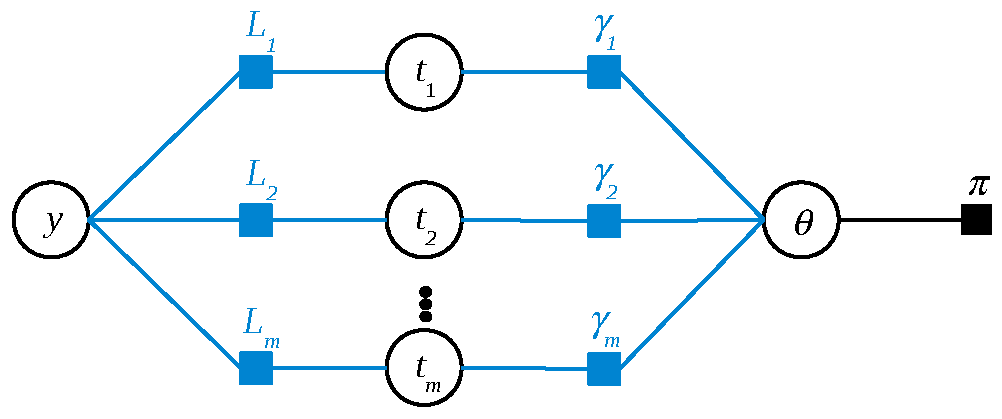
\includegraphics[width=.6\textwidth]{fgraph3.pdf}
  \end{center}
\caption{Alternative graph using population coding for the computation of $p(\theta|y)$. See text for details.}
\label{fig:fgraph3}
\end{figure}

The unnormalized joint distribution~$p_2(y,\theta)$ represented by the graph in Figure~\ref{fig:fgraph3} reads:
\begin{eqnarray*}
p_2(y,\theta) 
& = & 
\pi(\theta) \sum_{t_1=0}^{1}\ldots \sum_{t_m=0}^{1} 
\prod_{j=1}^m L_j(t_j) \gamma_j(t_j,\theta) \\
& = & 
\pi(\theta)  
\prod_{j=1}^m \left\{ 
\mathbf{1}_{\{\theta_j\}}(\theta) p(y|\theta_j) + [1-\mathbf{1}_{\{\theta_j\}}(\theta)]p(y|\theta_0)
\right\}\\
& = & 
\pi(\theta) p(y|\theta) p(y|\theta_0)^{m-1}
,
\end{eqnarray*}
clearly yielding the same posterior $p_2(\theta|y)=p(\theta|y)$ as the graph in Figure~\ref{fig:fgraph1}, although generally not the same generative model: $p_2(y|\theta)\propto p(y|\theta)p(y|\theta_0)^{m-1}$ hence $p_2(y|\theta)\not=p(y|\theta)$ unless there are two hypotheses only ($m=1$), or the null distribution~$p(y|\theta_0)$ is uniform. While the inconsistency between generative models is irrelevant to inference, the alternative graph enables a more flexible likelihood approximation scheme, where each factor $L_j(t_j)$ can be substituted with a specific composite likelihood $L_{cj}(t_j, \mathbf{w}_j)$ using own pre-determined weights $\mathbf{w}_j=(w_{1j},w_{2j},\ldots,w_{nj})^\top$ depending on~$j$:
$$
L_{cj}(t_j, \mathbf{w}_j) 
= \prod_{i=1}^n p(z_i|t_j)^{w_{ij}}
= \prod_{i=1}^n \beta_{ij}(z_i, t_j),
$$
with:
\begin{equation}
\label{eq:factor_beta}
\beta_{ij}(z_i, t_j)
= 
\left\{
\begin{array}{lll}
p(z_i|\theta_j)^{w_{ij}} = \ell_i (\theta_j)^{w_{ij}} & {\rm if} & t_j=1 \\
p(z_i|\theta_0)^{w_{ij}} = \ell_i (\theta_0)^{w_{ij}} & {\rm if} & t_j=0
\end{array}
\right.
,
\end{equation}
and:
$$
\forall j \in \{1,\ldots,m\},
\qquad
\sum_{i=1}^n w_{ij} = 1
.
$$

%Let $\mathbf{W}$ denote an $n\times m$ matrix of pre-determined unit sum weights $w_{ij}$ such that each column, denoted $\mathbf{w}_j$, sums up to one. The possibly sparse $\mathbf{W}$ encodes prior knowledge about the relative relevance of the selected clues to the different hypotheses under investigation. 

This corresponds to replacing each factor $L_j$ in Figure~\ref{fig:fgraph3} with a subgraph of same structure as the subgraph highlighted in red in Figure~\ref{fig:fgraph2}, resulting in the further modified factor graph shown in Figure~\ref{fig:fgraph4}. Intuitively, hypothesis-dependent weights make it possible to emphasize the clues that are relevant to each particular hypothesis comparison $\theta_j$ {\em vs.}~$\theta_0$, leading to potentially better approximations to the true odds $p(\theta_j|y)/p(\theta_0|y)$ than using constant weights.

\begin{figure}[!ht]
  \begin{center}
    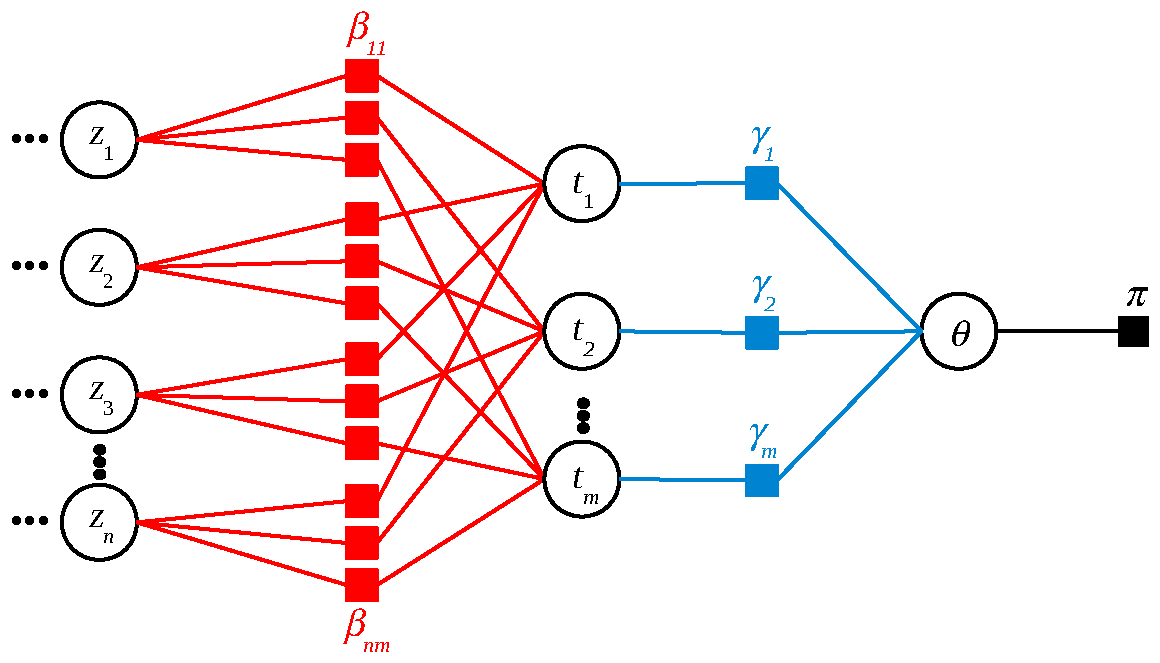
\includegraphics[width=.7\textwidth]{fgraph4.pdf}
  \end{center}
\caption{Super composite likelihood factor graph. See respectively (\ref{eq:factor_beta}) and (\ref{eq:factor_gamma}) for the expression of the factors $\beta_{ij}$ and  $\gamma_j$.}
\label{fig:fgraph4}
\end{figure}

We shall point out that the subgraph connecting ${\bf z}=(z_1,z_2,\ldots,z_n)$ and ${\bf t}=(t_1,t_2,\ldots,t_m)$ in Figure~\ref{fig:fgraph4} (shown in red) is equivalent to an undirected bipartite graph, a property shared with restricted Boltzmann machines (RBM) \cite{Fischer-14,Hinton-06,Larochelle-08}. This means that the variables in one layer are independent conditionally on the other layer:
\begin{equation}
\label{eq:bipartite}
p_3({\bf t}|{\bf z}) = \prod_{j=1}^m p_3(t_j|{\bf z}),
\qquad
p_3({\bf z}|{\bf t}) = \prod_{i=1}^n p_3(z_i|{\bf t}),
\end{equation}
with, in this case, 
$$
p_3(t_j|{\bf z}) \propto L_{cj}(t_j, \mathbf{w}_j),
\qquad
p_3(z_i|{\bf t}) = p_3(z_i|\theta) \propto p(z_i|\theta)^{W_i(\theta)},
$$
where $W_i(\theta)$ is defined by $W_i(\theta_j)=w_{ij}$ if $j\in\{1,m\}$ and $W_i(\theta_0)=\sum_{j=1}^m w_{ij}$.

% and may hence be considered as a kind of restricted Boltzmann machine (RBM) \cite{Fischer-14,Hinton-06,Larochelle-08}: specifically, one with real-valued (or even vector-valued) inputs and truncated binary outputs. The parameters of this RBM are the feature sampling distribution parameters as well as the weights~${\bf W}$. Assuming that the former are known, there is a very natural method to learn~${\bf W}$, as we will see in Section~\ref{sec:weights}, which differs from traditional RBM~learning methods, namely contrastive and discriminative learning.

An essential difference with RBM, however, is that the generative distribution $p_3({\bf z}|{\bf t})$ is not intended to be used for model training. Instead, our core assumption is that the marginal feature distributions are learned ``before'' constructing the graph, a step that does not rely on assuming feature independence conditionally on~${\bf t}$ or, equivalently, $\theta$. Therefore, despite satisfying the bipartite condition (\ref{eq:bipartite}), the joint distribution $p_3({\bf t},{\bf z})$ represented in Figure~\ref{fig:fgraph2} is asymmetrical in use, and serves the only purpose of defining a posterior distribution~$p_3(\theta|y)$ via~$p_3({\bf t}|{\bf z})$.

Marginalizing out~${\bf t}$, we find:
\begin{eqnarray*}
p_3(\theta|y) 
& \propto & 
\pi(\theta) \sum_{{\bf t}\in \{0,1\}^m} 
\prod_{j=1}^m p_3({\bf t}|{\bf z}) \gamma_j(t_j,\theta) \\
& = & 
\pi(\theta) \sum_{t_1=0}^{1}\ldots \sum_{t_m=0}^{1} 
\prod_{j=1}^m L_{cj}(t_j, \mathbf{w}_j) \gamma_j(t_j,\theta) \\
& = & 
\pi(\theta) 
\prod_{i=1}^n
\prod_{j=1}^m
\ell_i \left(
\mathbf{1}_{\{\theta_j\}}(\theta) \theta + [1-\mathbf{1}_{\{\theta_j\}}(\theta)]\theta_0
\right)^{w_{ij}} \\
& = & 
\pi(\theta) 
\prod_{i=1}^n \ell_i(\theta_0)^{\sum_{j=1}^m w_{ij}}
\prod_{i=1}^n \left[
\frac{\ell_i(\theta)}{\ell_i(\theta_0)}
\right]^{w_{ij}}
,
\end{eqnarray*}
therefore:
\begin{equation}
\label{eq:new_pool}
p_3(\theta|y) 
=
K \frac{\pi(\theta)}{\pi(\theta_0)}
\prod_{i=1}^n \left[
\frac{\ell_i(\theta)}{\ell_i(\theta_0)}
\right]^{w_i(\theta)},
\end{equation}
where $K$ is a normalizing factor (dependent on~$y$) and the functions $w_i(\theta)$ are defined by $w_i(\theta_j)=w_{ij}$ for $j=1,\ldots,m$ and $w_i(\theta_0)=0$ conventionally. 

As an opinion pooling rule, (\ref{eq:new_pool}) is more general than the log-linear pool~(\ref{eq:log_pool}) as it explicitly depends on~$\theta$ through the changing weights. Moreover, since the weights sum up to one for each~$\theta\not=\theta_0$, we have the equivalent expression:
$$
p_3(\theta|y) 
=
K
\prod_{i=1}^n \left[
\frac{\pi(\theta)\ell_i(\theta)}{\pi(\theta_0)\ell_i(\theta_0)}
\right]^{w_i(\theta)},
$$
showing that the pool does not change depending on whether the prior is incorporated before or after combining experts. In other words, (\ref{eq:new_pool}) is, again, externally Bayesian.

As in Section~\ref{sec:pool}, we recognize a Bayes rule-type expression: $p_3(\theta|y)\propto\pi(\theta){\cal L}_c(\theta,\mathbf{W})$, with:
\begin{equation}
\label{eq:super}
{\cal L}_c(\theta,\mathbf{W})
\equiv
\prod_{i=1}^n \left[
\frac{\ell_i(\theta)}{\ell_i(\theta_0)}
\right]^{w_i(\theta)}
,
\end{equation}
where~$\mathbf{W}$ denotes the $n\times m$ weight matrix with general element $w_{ij}$. We call~(\ref{eq:super}) a super composite likelihood (SCL). Note that the SCL evaluated at a particular hypothesis~$\theta_j$ boils down to a composite likelihood ratio,
\begin{equation}
\label{eq:super_ratio}
{\cal L}_c(\theta_j,\mathbf{W}) = 
\frac{L_c(\theta_j,\mathbf{w}_j)}{L_c(\theta_0,,\mathbf{w}_j)}
.
\end{equation}

To see that SCL~(\ref{eq:super}) is indeed a generalization of composite likelihood, assume that $\mathbf{w}_j=\mathbf{w}$ is the same for all hypotheses. This implies that (\ref{eq:super_ratio}) simplifies to ${\cal L}_c(\theta,\mathbf{W})=L_c(\theta,\mathbf{w})/L_c(\theta_0,\mathbf{w})$, the denominator of which is independent from~$\theta$ and can therefore be safely ignored for inference about~$\theta$. In this special case, SCL is equivalent to standard composite likelihood regardless of the chosen reference~$\theta_0$.

Nevertheless, $\theta_0$ plays a crucial normalization role whenever the columns of $\mathbf{W}$ are different to enable complex, possibly sparse, weighting patterns. Consider, for instance, the case where each hypothesis gets evidence from a single clue, so that $\mathbf{W}$ has a single~1 in each column and all other elements~0. The SCL~(\ref{eq:super}) then reduces to a likelihood ratio involving a single, hypothesis-specific clue $z_{\iota(j)}$ determined by some mapping $\iota:\{1,\ldots,m\}\to \{1,\ldots,n\}$:
\begin{equation}
\label{eq:pdf_proj}
{\cal L}_c(\theta_j,\mathbf{W})
= \frac{\ell_{\iota(j)}(\theta_j)}{\ell_{\iota(j)}(\theta_0)}
= \frac{p(z_{\iota(j)}|\theta_j)}{p(z_{\iota(j)}|\theta_0)}
.
\end{equation}

This expression was already used in \cite{Baggenstoss-03,Minka-04,Baggenstoss-15} motivated by a different argument than here, namely the {\em PDF projection theorem}, which states the full data-generating model maximizing relative entropy (with respect to a chosen reference distribution) under knowledge of the feature sampling distributions. As discussed in \cite{Baggenstoss-03}, (\ref{eq:pdf_proj}) closely approximates the true likelihood if each $z_{\iota(j)}$ is a near-sufficient statistic for~$\theta_j$ {\em vs.}~$\theta_0$, a condition that may be difficult to meet if the choice of clues is driven by computational efficiency. SCL provides an alternative interpretation of PDF~projection, while also extending it to multiple clues with unknown statistical dependences.


\section{Weight optimization}
\label{sec:weights}

The general advantage of~SCL over standard composite likelihood is to define a broader class of pseudo-likelihood functions, hence with the potential to better approximate the true likelihood for a suitable choice of the weight matrix~$\mathbf{W}$. On the other hand, standard composite likelihood satisfies good asymptotic properties for any choice of unit sum positive weights, as shown in Appendix~\ref{sec:asymptotic}, but such properties do not extend in full generality to~SCL: a poor likelihood approximation is to be expected if~$\mathbf{W}$ is chosen at random, hence the importance of fine-tuning super composite weights.

To this end, a conventional machine learning strategy may be used. Assume (for now) that a number of examples of inputs and responses $(y^k, \theta^k)$, for $k=1,\ldots,N$, are sampled independently. Given a tentative weight matrix~$\mathbf{W}$, examples elicit different SCL functions ${\cal L}_{ck}(\theta, \mathbf{W})$ as $y^k$ varies across examples. By analogy with classical maximum likelihood model selection, we may consider rating the model ability to predict examples depending on~$\mathbf{W}$ via the sample average logarithm of the~SCL:
\begin{eqnarray*}
\hat{\cal U}(\mathbf{W})
& = & 
\frac{1}{N} \sum_{k=1}^N \log {\cal L}_{ck}(\theta^k, \mathbf{W})\\
& = &  
\frac{1}{N} \sum_{k=1}^N \sum_{i=1}^n w_i(\theta^k) \log \frac{p(z_i^k|\theta^k)}{p(z_i^k|\theta_0)}
,
\end{eqnarray*}
which essentially averages feature-based log-likelihood ratios relative to the chosen reference hypothesis~$\theta_0$.

This utility measure turns out to be particularly appealing to tune SCL weights, for two reasons. First, if examples are drawn from the true yet incompletely known joint distribution $p(y,\theta)=\pi(\theta)p(y|\theta)$, then, under the condition of existence, $\hat{\cal U}(\mathbf{W})$ converges in the limit of many examples to:
\begin{eqnarray}
{\cal U}(\mathbf{W})
& = & 
E\left[
\log {\cal L}_c(\theta, \mathbf{W})
\right] \nonumber \\
& = & 
\sum_{j=1}^m \pi(\theta_j) \sum_{i=1}^n w_{ij} 
\underbrace{\int p(z_i|\theta_j) \log \frac{p(z_i|\theta_j)}{p(z_i|\theta_0)} dz_i}_{u_{ij}},
\label{eq:discrim}
\end{eqnarray}
where $u_{ij}$ denotes the KL~divergence of~$p(z_i|\theta_0)$ from~$p(z_i|\theta_j)$, and can be interpreted as the utility of clue~$i$ regarding hypothesis~$j$. Since the $u_{ij}$'s are fully determined by the known feature-generating distributions~$p(z_i|\theta)$, (\ref{eq:discrim}) can be evaluated without further knowledge about~$p(y,\theta)$. Consequently, we do not need to constitute an actual training dataset! 

Second, let~${\cal U}_\star$ denote the expected utility associated with the true distribution~$p(y,\theta)$, considered as a SCL built from a single clue, the full data~$y$. As is easy to check, ${\cal U}_\star$ is the conditional Kullback-Leibler divergence of~$p(y|\theta_0)$ from~$p(y|\theta)$:
$$
{\cal U}_\star
= \sum_{j=1}^m \pi(\theta_j) \int p(y|\theta_j) \log \frac{p(y|\theta_j)}{p(y|\theta_0)} dy
= D[p(y|\theta)\|p(y|\theta_0)]
.
$$

Applying in~(\ref{eq:discrim}) the data reduction inequality recalled in Appendix~\ref{sec:reduction_inequality}, we obtain the intuitive result that~${\cal U}(\mathbf{W})$ is upper bounded by the expected utility achievable without data reduction: 
$$
{\cal U}(\mathbf{W})\leq {\cal U}_\star
.
$$
This means that the full data-generating model maximizes the expected log-SCL over the whole space of SCL functions ({\em i.e.}, SCL functions built from arbitrary clues in arbitrary number and using arbitrary weights). Therefore, (\ref{eq:discrim}) qualifies as a measure of goodness of fit to the true likelihood. 

Maximizing~(\ref{eq:discrim}) with respect to~$\mathbf{W}$ amounts to optimizing the fit over a subspace of SCL functions spanned by fixed user-specified features. Some constraints may be imposed on~$\mathbf{W}$, such as assuming identical columns as in the case of standard composite likelihood, or forcing some elements to zero if some feature likelihood functions are only known on subsets of~$\Theta$. We here focus on the case where no constraints are imposed beside, of course, that the columns of~$\mathbf{W}$ lie in the $n$-dimensional simplex. Clearly, the optimal weights are then determined independently for each hypothesis (and thus independently from the prior) as any positive weights satisfying, for all~$j\in\{1,\ldots,n\}$:
\begin{equation}
\label{eq:optimal_weights}
w_{ij} = 0 
\quad {\rm iff}\quad  
i \not\in \arg\max_{i'\in\{1,\ldots,n\}} u_{i'j},
\qquad {\rm and} \quad
\sum_{i=1}^n w_{ij}=1
,
\end{equation}
yielding a sparsity-enforcing rule which assigns non-zero weights only to the clues that achieve maximal KL~utility for a particular hypothesis. If there is a unique KL-maximal, or ``most exhaustive'' clue for each hypothesis, the resulting~SCL function essentially boils down to the PDF~projection method \cite{Baggenstoss-03,Minka-04,Baggenstoss-15}. More generally, if several clues~$z_i$ maximize $u_{ij}$ for some hypothesis~$\theta_j$, then optimal weights are not unique. In such case, it is preferable to assign equal weights to the winning clues in order to ensure that utility is not only large in average, but also stable across examples ({\em i.e.}, low in variance). 

Also note that the weight optimality rule~(\ref{eq:optimal_weights}) implies that, for any $\theta_\star \in \Theta$,
$$
E\left[ \log \frac{L_c(\theta_\star, \mathbf{w})}{L_c(\theta_0, \mathbf{w})} \right]
\leq
E\left[ \log \frac{L_c(\theta_\star, \mathbf{w}_\star)}{L_c(\theta_0, \mathbf{w}_\star)} \right],
$$
where $\mathbf{w}_\star$ is the weight vector associated with~$\theta_\star$, $E$ stands for the expectation with respect to $p(y|\theta_\star)$, and~$\mathbf{w}$ is any weight vector. Moreover, the following inequality is shown in Appendix~\ref{sec:asymptotic}:
$$
E\left[ \log \frac{L_c(\theta, \mathbf{w})}{L_c(\theta_0, \mathbf{w})} \right]
\leq
E\left[ \log \frac{L_c(\theta_\star, \mathbf{w})}{L_c(\theta_0, \mathbf{w})} \right]
,
$$
for any hypothesis~$\theta$ and weighting~$\mathbf{w}$ and, in particular, for the weight vector associated with~$\theta$ via~(\ref{eq:optimal_weights}). Therefore, provided that the weight matrix~$\mathbf{W}$ verifies~(\ref{eq:optimal_weights}), we have that:
$$
E \left[\log {\cal L}_c(\theta,\mathbf{W}) \right]
\leq 
E \left[\log {\cal L}_c(\theta_\star,\mathbf{W}) \right]
,
$$
meaning that the SCL is asymptotically consistent in the sense that the expectation of its logarithm is maximized by the ``true'' parameter value. This is a most awaited frequentist property which, as already pointed out, holds with any choice of weights for standard composite likelihood but not, in general, for~SCL.

%Regularized version.
%$$
%{\cal U}_\gamma(\mathbf{W})
%= \sum_{j=1}^m \pi(\theta_j) \sum_{i=1}^n (w_{ij}u_{ij}-\frac{\gamma}{2}w_{ij}^2)
%$$
%$\gamma>0$ is a constant. Maximizing this leads to independent quadratic programming problems for each~$j$. Can be solved using standard numerical methods \cite{Nocedal-99}. As $\gamma\to 0$, the optimal weights are uniform among clues satisfying (\ref{eq:optimal_weights}).


\section{Further extensions}

\subsection{Conditional super composite likelihood}
\label{sec:conditional}

The SCL derivation rests upon the definition of feature-based likelihood as $\ell_i(\theta)=p(z_i|\theta)$. As a straightforward  extension, $\ell_i(\theta)$ may be conditioned by an additional ``independent'' feature $z^c_i = f^c_i(y)$ considered as a predictor of the ``dependent'' feature, $z_i=f_i(y)$, yielding the more general form:
\begin{equation}
\label{eq:cond_feat_lik}
\ell_i(\theta) = p(z_i|\theta,z^c_i).
\end{equation}

Conditioning may be useful if it is believed that $z^c_i$ alone is little or not informative about $\theta$, but can provide relevant information when considered jointly with $z_i$, as in the case of regression covariates, for instance. Standard composite likelihood (\ref{eq:comp_lik}) then amounts to {\em conditional composite likelihood} \cite{Varin-11}, a more general form of composite likelihood also including Besag's historical {\em pseudo-likelihood} \cite{Besag-74}, which was a major breakthrough in computer vision. 

Likewise, the above derivation remains valid when ``independent'' features are used, and we can thus define a conditional version of SCL by plugging likelihood functions of the form~(\ref{eq:cond_feat_lik}) into (\ref{eq:super}).


\subsection{Nuisance parameters}
\label{sec:nuisance_params}

Most often, plausible feature-generating models involve unknown quantities of no direct interest. Such quantities may be estimated offline in a supervised learning phase if a suitable training dataset is available. However, if such ``pre-training'' is not feasible in practice, the feature-based likelihoods depend on an unknown parameter~$\psi$, in addition to the parameter of interest~$\theta$:  $\ell_i(\theta,\psi)=p(z_i|\theta,\psi)$, or $\ell_i(\theta,\psi)=p(z_i|z^c_i,\theta,\psi)$ if ``independent'' features are used. We then face two difficulties: 
\begin{itemize}
\item {\em Parameter integration.} How to make the inference on~$\theta$ independent from~$\psi$ assuming known SCL~weights?
\item {\em Weight optimization.} How to optimize the SCL~weights under unknown~$\psi$?
\end{itemize}

We address these two points in the sequel.

%We may then seek a means to eliminate~$\psi$.

\subsubsection{Parameter integration}
\label{sec:nuisance_integration}

When weighting clues independently from the hypotheses, a joint composite likelihood on both parameters may be derived:
$$
L_c(\theta,\psi,\mathbf{w}) = \prod_i \ell_i(\theta,\psi)^{w_i},
$$
and further integrated with respect to some prior on the nuisance parameter to yield a function of~$\theta$ only, which we may call the {\em composite evidence}:
\begin{equation}
\label{eq:comp_evidence}
\bar{L}_c(\theta, \mathbf{w}) = \int \pi(\psi) L_c(\theta,\psi,\mathbf{w}) d\psi
.
\end{equation}
This corresponds to using the factor graph represented in Figure~\ref{fig:fgraph5} to approximate the message from the data to~$\theta$, where the factors $\beta_i$ are now defined by $\beta_i(z_i,\theta,\psi)=\ell_i(\theta,\psi)^{w_i}$. To compute the associated posterior $p_4(\theta|y)$, $\psi$ is treated as an auxiliary variable to be integrated out, leading to $p_4(\theta|y)\propto \pi(\theta)\bar{L}_c(\theta, \mathbf{w})$.

\begin{figure}[!ht]
  \begin{center}
    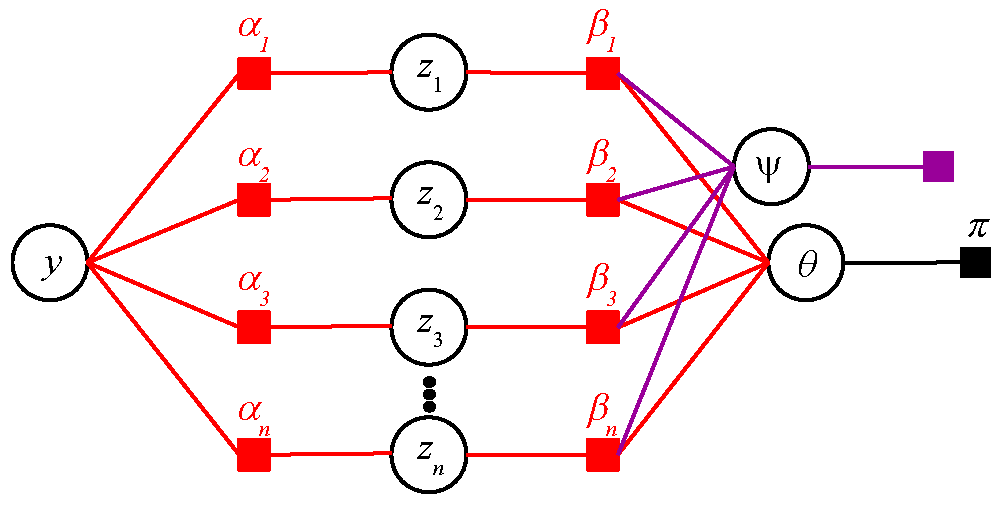
\includegraphics[width=.6\textwidth]{fgraph5.pdf}
  \end{center}
\caption{Extension of the composite likelihood factor graph in Figure~\ref{fig:fgraph2} to account for nuisance parameters.}
\label{fig:fgraph5}
\end{figure}

More generally, when weighting clues depending on hypotheses, we may use essentially the same idea as in Section~\ref{sec:super}, {\em i.e.}, replicate subgraphs such as the one depicted in red and magenta in Figure~\ref{fig:fgraph5} in order to approximate the different messages sent from the data to each truncated variable~$t_j$, as defined in~(\ref{eq:binary}). Note that, by replicating the same graph structure across variables~$t_j$, the variable~$\psi$ is also replicated, so that the resulting factor graph in Figure~\ref{fig:fgraph6} does not represent a joint distribution of the form $p(y,\theta,\psi)$, but rather one of the form~$p(y,\theta,\psi_1,\ldots,\psi_m)$. This makes the approximation more flexible by taking advantage of the fact that a marginal distribution on~$\psi$ is not required.

\begin{figure}[!ht]
  \begin{center}
    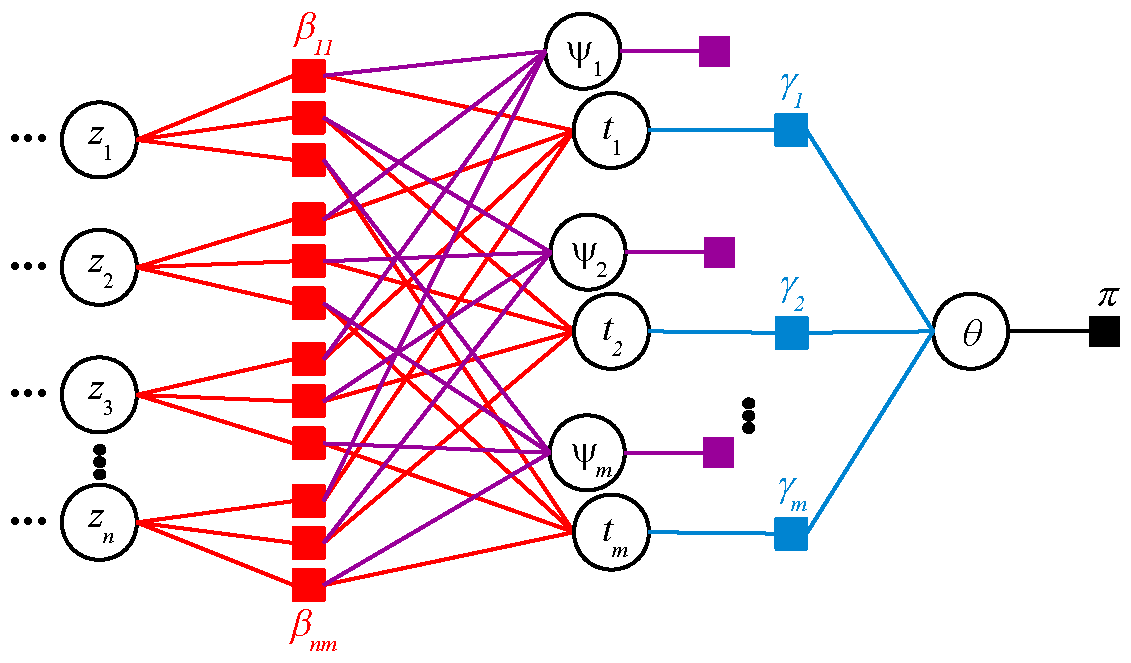
\includegraphics[width=.7\textwidth]{fgraph6.pdf}
  \end{center}
\caption{Extension of the super composite likelihood factor graph in Figure~\ref{fig:fgraph4} to account for nuisance parameters. Here, the factors $\beta_{ij}(z_i,t_j,\psi_j)$ are defined by $\beta_{ij}(z_i,1,\psi_j)=\ell_i(\theta_j,\psi_j)^{w_{ij}}$ and $\beta_{ij}(z_i,0,\psi_j)=\ell_i(\theta_0,\psi_j)^{w_{ij}}$.}
\label{fig:fgraph6}
\end{figure}

The posterior distribution encoded by this graph (integrated with respect to the replicates $\psi_1,\ldots,\psi_m$) is easily found to be:
$$
p_5(\theta|y)
\propto
\pi(\theta)
\left\{
\begin{array}{lll}
\displaystyle
\frac{\bar{L}_c(\theta_j,\mathbf{w}_j)}{\bar{L}_c(\theta_0,\mathbf{w}_j)} & {\rm if} & \theta=\theta_j \quad {\rm with} \quad j\in\{1,\ldots,m\}\\
1 & {\rm if} & \theta=\theta_0
\end{array}
\right.
,
$$
where $\bar{L}_c(.,\mathbf{w}_j)$ is the above-defined composite evidence function~(\ref{eq:comp_evidence}) associated with the weight vector~$\mathbf{w}_j$. This justifies defining the {\em super composite evidence} as:
\begin{equation}
\label{eq:super_comp_evidence}
\bar{\cal L}_c(\theta_j,\mathbf{W}) = 
\left\{
\begin{array}{lll}
\displaystyle
\frac{\bar{L}_c(\theta_j,\mathbf{w}_j)}{\bar{L}_c(\theta_0,\mathbf{w}_j)} & {\rm if} & j\in\{1,\ldots,m\}\\
1 & {\rm if} & j=0
\end{array}
\right.
.
\end{equation}

Obvious from~(\ref{eq:super_comp_evidence}) is that the super composite evidence conserves all odds $\theta_j$ {\em vs.}~$\theta_0$ integrated within their respective associated subgraphs, very much like its nuisance parameter-free version~(\ref{eq:super_ratio}). The conservation of odds implies  that evaluating the SCL at a particular~$\theta$ is akin to computing a scaled Bayes factor, which may sometimes be efficiently approximated via a maximum likelihood ratio statistic.

%The philosophical question, maybe, is whether it's better to approximate the integrated likelihood, or integrate the approximated likelihood. 

\subsubsection{Weight optimization}
\label{sec:nuisance_weights}

Consistently with the idea of nuisance parameter replication (see Figure~\ref{fig:fgraph5}), we may employ a nested strategy to optimize the SCL~weights in presence of nuisance parameters: for each $j\in\{1,\ldots,m\}$, apply the weight optimization of Section~\ref{sec:weights} to the  subgraph model connecting all clues~$z_i$ with the particular pair $(t_j,\psi_j)$. This leads to a set of linear programming problems: for each~$j$, find the weight vector~${\bf w}_j$ on the $n$-dimensional simplex that maximizes:
$$
\bar{\cal U}_j({\bf w}_j) 
= 
E\left[\log \frac{L_c(\theta_j,\psi_j,{\bf w}_j)}{L_c(\theta_0,\psi_j,{\bf w}_j)}\right],
$$
where the expectation is taken with respect to $(y,\psi_j)\sim p(y|\theta_j,\psi)\pi(\psi)$, a computation that only requires knowledge of the feature sampling distributions, $p(z_i|\theta,\psi)$ for $i=1,\ldots,n$, in addition to the prior $\pi(\psi)$.

In this way, every ${\bf w}_j$ is optimal for the posterior of~$(t_j,\psi_j)$ or, more precisely, yields the best approximation to the true joint likelihood $L(\theta, \psi)$ for~$\theta$ restricted to the binary set~$\{\theta_0,\theta_j\}$. The ensuing marginal likelihood approximations are therefore as tight as possible for all hypothesis comparisons with~$\theta_0$, as is the goal of SCL~weight optimization. 

% En clair, c'est l'idee du college d'experts travaillant sur une hypothese binaire et integrant les parametres de nuisance sans tenir compte de ce que font les autres. 


\section{Discussion}
\label{sec:discussion}

Composite likelihood is a relatively recent concept from computational statistics that has mainly been developed so far in a frequentist perspective as a surrogate for the maximum likelihood method. In this paper, we have shown (to our best knowledge, for the first time) a deep connection between composite likelihood and  probabilistic opinion pooling, thereby establishing composite likelihood as a class of {\em discriminative models}\footnote{We here define a discriminative model as a model of which the parameters describe the conditional distribution of an unobserved variable of interest given an observable variable, as opposed to a {\em generative} model, which involves parameters encoding for the conditional distribution of an observable given an unobserved variable.} for statistical inference and machine learning. This connection is possible under the mild restriction that composite likelihood weights are chosen to sum up to one.

\subsection{From na\"ive Bayes to super composite likelihood}

In the probabilistic opinion pooling perspective, composite likelihood is essentially a reinterpretation and a generalization of the {\em na\"ive Bayes} paradigm that relaxes the associated ``na\"ive'' mutual feature independence assumption. In particular, when all features are given equal weight, the composite likelihood is the na\"ive Bayes likelihood raised to the power~$1/n$, where~$n$ is the number of selected features, yielding for instance the same maximum a posteriori (MAP) estimator if a flat prior is used. However, beside providing a simple justification to the wide use of na\"ive Bayes MAP algorithms,  composite likelihood using unit sum weights also entails a conservative rescaling of credibility sets derived from na\"ive Bayes, which gets more drastic as the number of features increases. This comes as a consequence of relaxing feature independence.

We further argued that this rescaling may, to some extent, be unduly conservative in multiclass problems if features are weighted uniformly over the space of unobserved labels, leading us to propose the more general concept of super composite likelihood (SCL). SCL essentially approximates likelihood ratios relative to a fixed reference hypothesis using locally weighted composite likelihood functions. Owing to weight adaptability, SCL describes a more general class of discriminative models than standard composite likelihood. 

The idea can also be understood in terms of approximating the factor graph in Figure~\ref{fig:fgraph3}, which encodes the true but intractable posterior distribution, by another factor graph of the type depicted in Figure~\ref{fig:fgraph4}. This substitution results in breaking into pieces both the observed and unobserved variable spaces, and assembling a series of concise {\em messages} passing from the former to the latter. Note that this is a pretty unusual case of approximate inference in factor graphs where the factors to be approximated are unknown (or need not be known).

\subsection{Super composite likelihood training}

Any SCL~model is fully determined by the marginal generative distributions of some pre-specified features, which may rely on a moderate number of parameters if low-dimensional features are chosen. There are two approaches to deal with these parameters.

One is to estimate them beforehand by supervised learning, if an adequate training dataset is available. This could be compared with contrastive pre-training of RBMs \cite{Hinton-06,Fischer-14}, which also optimizes parameters for generation of observable features. An important difference, however, is that contrastive pre-training is unsupervised. On the other hand, SCL pre-training relies on weaker assumptions as it does not assume conditional feature independence unlike RBMs. Once pre-training is complete, the SCL~weights may be tuned by maximum~SCL, as shown in Section~\ref{sec:weights}: this second training stage is, again, supervised in essence, but does not require additional training examples since it is fully determined by the feature distributions learned in the pre-training step.

%{\color{red} Moreover, while RBM parameters are typically refined in a supervised discriminative learning step, disjoint set of parameters for SCL. Dunno how to say that.} 

%In such context, SCL competes with classical discriminative models (logistic regression, Gaussian processes \cite{Rasmussen-06}, maximum entropy models \cite{BergerA-96}, etc.), and may compare more or less favorably in practice depending on the amount of training data. For relatively small training datasets, we may hope for more accurate inference using~SCL than using traditional discriminative models, extrapolating from the results of \cite{Ng-01} regarding the comparison between logistic regression and na\"ive Bayes classifiers.
%{\color{red}Ici, il manque la comparaison avec les RBMs qui ne sont pas (forcement) des modeles discriminatifs.}

\begin{figure}[!ht]
\begin{center}
\subfigure[Generative model]{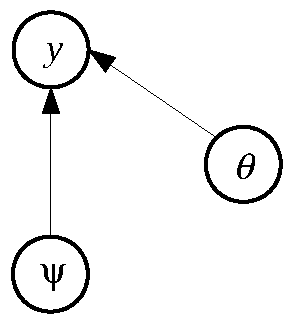
\includegraphics[width=.25\textwidth]{dgraph1.pdf}\label{fig:dgraph1}}
\hspace*{.05\textwidth}
\subfigure[Classical discriminative model]{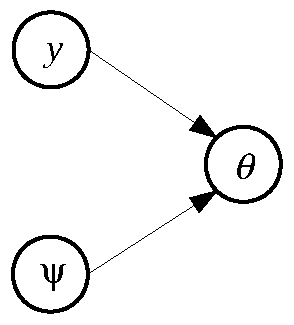
\includegraphics[width=.25\textwidth]{dgraph2.pdf}\label{fig:dgraph2}}
\hspace*{.05\textwidth}
\subfigure[Composite likelihood model]{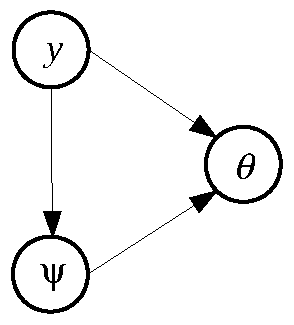
\includegraphics[width=.25\textwidth]{dgraph3.pdf}\label{fig:dgraph3}}
\caption{Belief networks representing, respectively: (a) a generative model, (b) a classical discriminative model, and (c) a composite likelihood model. Note the marginal independence between the data~$y$ and the nuisance parameter~$\psi$ in (b).}
\label{fig:dgraph}
\end{center}
\end{figure}

%%, hence alleviating the need for heavily supervised model training

The other approach to deal with feature distribution parameters is to consider them as nuisance parameters, as proposed in Section~\ref{sec:nuisance_params}, thereby avoiding pre-training. The method then becomes completely unsupervised. The weights can be tuned by maximizing the log-SCL integrated over the prior on nuisance parameters (see Section~\ref{sec:nuisance_weights}), which requires no training dataset whatsoever, and the nuisance parameters can be eliminated by substituting the~SCL function with a {\em super composite evidence} (see Section~\ref{sec:nuisance_integration}). In this version, SCL~essentially generalizes Bayesian integration. 

The potential of SCL for unsupervised learning is perhaps suprising considering that it is a discriminative model. This stems from the fact that, unlike classical discriminative models, SCL~exploits direct information conveyed by the data about both the parameters of interest and the nuisance parameters, reflecting the generative nature of the underlying feature distribution models. This essential difference is illustrated in Figure~\ref{fig:dgraph}: the factor graph model underlying composite likelihood in its parametric version (see Figure~\ref{fig:fgraph5}) is not reducible to a belief network of the type represented in Figure~\ref{fig:dgraph2}, in which the data and the nuisance parameter are marginally independent. In contrast, the data is informative about the nuisance parameter in a composite likelihood model, as shown in Figure~\ref{fig:dgraph3}.


\section{Conclusion}
\label{sec:conclusion}

In summary, (super) composite likelihood has the potential to yield weakly supervised or unsupervised Bayesian-like inference procedures depending on the particular task at hand. This property reflects the encoding of statistical relationships between the data and {\em all} unknown parameters. Composite likelihood thus appears as a trade-off between generative models, which are optimal for unsupervised learning but possibly intractable, and traditional discriminative models (logistic regression, Gaussian processes \cite{Rasmussen-06}, maximum entropy models \cite{BergerA-96}, etc.), which are inherently supervised. Composite likelihood models are discriminative models assembled from atomic generative models and, from this point of view, may be considered as {\em semi-generative} models.



%composite likelihood may be considered as a {\em semi-generative} model: a discriminative model assembled from partial generative models.

%As a note of caution, we shall stress that the pre-determined weights assigned to the different associations between observed and unobserved values represent prior knowledge regarding the informativeness of clues. A poor choice of weights will inevitably result in a poor approximation to the ``true'' Bayesian posterior -- the posterior that would be obtained from a realistic generative model if it was tractable. In future work, we will investigate feature selection strategies to mitigate this problem.

% Improve the discussion on following aspects:
% ** Why is it compatible with unsupervised learning? Give more insight.
% ** Stress the contribution: class-specific weighting.
% * Pivotality argument.
% * Bayes is a special case of composite Bayes.

%{\color{red} {\em Mardi 12 avril 2016.} Je laisse reposer la version actuelle 3-4 semaines avant mise \`a jour sur arxiv. La plupart des points qui restaient obscurs en f\'evrier ont, me semble-t-il, \'et\'e lev\'es: lien avec les neural networks/RBM, strat\'egies d'apprentissage, optimisation des poids, int\'er\^et du super composite (multi-class problems). Sur l'optimisation des poids, il reste une petite zone d'ombre: faut-il r\'egulariser d'apprentissage de mani\`ere \`a \'eviter une pond\'eration \'eparse? L'argument pour serait d'acc\'el\'erer la convergence stochastique de la SCL vers l'utilit\'e th\'eorique. On en parle d\'ej\`a un peu dans la version actuelle en disant que si 2 attributs sont aussi informatifs l'un que l'autre, alors le mieux est de leur donner le m\^eme poids. Plus g\'en\'eralement, on pourrait aborder cet aspect via: 1) des contraintes de r\'epartition ``d\'emocratique'' des poids pour \'eviter une situation ``winner-take-all'' (eg, avec une p\'enalisation quadratique des poids); ou alors, 2) des contraintes de variations impos\'ees aux colomnes de la matrice de poids, ce qui donnerait une esp\`ece de compromis entre CL classique et SCL... mais je ne suis pas certain de l'int\'er\^et.}


\appendix

\section{Data reduction inequality}
\label{sec:reduction_inequality}

A fundamental property of the Kullback-Leibler divergence is that it decreases under feature extraction, {\em i.e.}, application of a deterministic transformation. This comes as a consequence of the logarithmic sum inequality \cite{Cover-06} (and also follows as a straightforward corollary of the PDF~projection theorem \cite{Minka-04,Baggenstoss-15}). 

The proof is elementary and can be sketched as follows. Let $Z=f(Y)$ some feature extracted from a variable~$Y\sim p(y)$. Given an arbitrary distribution~$\pi(y)$, let  $\tilde{p}(z)$ and $\tilde{\pi}(z)$ the distributions induced on~$Z$ by $p(y)$ and $\pi(y)$, respectively. For any potential value~$z$ of~$Z$, consider the level set: $\Gamma(z)=\{y, f(y)=z\}$. Under conditions of existence, we can partition the integral involved in the KL~divergence $D(p\|\pi)$ using these level sets: 
$$
\int p(y) \log \frac{p(y)}{\pi(y)} dy
=
\int \left( \int_{\Gamma(z)} p(y) \log \frac{p(y)}{\pi(y)} dy \right) dz\\
.
$$

Applying the logarithmic sum inequality \cite{Cover-06} to each integral over~$\Gamma(z)$, we then readily get:
$$
\int_{\Gamma(z)} p(y) \log \frac{p(y)}{\pi(y)} dy
\geq 
\tilde{p}(z) \log \frac{\tilde{p}(z)}{\tilde{\pi}(z)}
,
$$
owing to the fact that $\displaystyle \int_{\Gamma(z)} p(y) dy = \tilde{p}(z)$ by definition. Therefore,
$$
\int \tilde{p}(z) \log \frac{\tilde{p}(z)}{\tilde{\pi}(z)} dz
\leq 
\int p(y) \log \frac{p(y)}{\pi(y)} dy
,
$$
or, in a more compact way, $D(\tilde{p}\|\tilde{\pi})\leq D(p\|\pi)$. The case of equality occurs if, and only if, $p(y)/\pi(y)=\tilde{p}(z)/\tilde{\pi}(z)$, in other words, if~$z$ is a sufficient statistic for the ``alternative'' hypothesis~$H_1:y\sim p(y)$ versus the ``null'' hypothesis~$H_0:y\sim\pi(y)$. 

Since it is a well-known fact that $D(\tilde{p}\|\tilde{\pi})\geq 0$ as any KL~divergence, we conclude that:
\begin{equation}
\label{eq:reduction_inequality}
0 
\leq D(\tilde{p}\|\tilde{\pi}) 
\leq D(p\|\pi)
.
\end{equation}


\section{Basic asymptotic properties of composite likelihood}
\label{sec:asymptotic}

It follows from the double inequality~(\ref{eq:reduction_inequality}) that, for any extracted feature~$z_i$ and for any hypothesis~$\theta$,
$$
0 \leq
E\left[
\log \frac{p(z_i|\theta_\star)}{p(z_i|\theta)}
\right]
\leq
E\left[
\log \frac{p(y|\theta_\star)}{p(y|\theta)}
\right],
$$
where the expectation is taken with respect to the true distribution $p(y|\theta_\star)$. Using a weighted sum of such inequalities, we can bracket the expected variations of the logarithm of any standard composite likelihood function (assuming unit sum positive weights):
\begin{equation}
\label{eq:variation_bound}
0 \leq
E\left[ \log \frac{L_c(\theta_\star, \mathbf{w})}{L_c(\theta, \mathbf{w})} \right]
\leq 
E\left[ \log \frac{L(\theta_\star)}{L(\theta)} \right]
.
\end{equation}

This implies two asymptotic properties of standard composite likelihood: 
\begin{itemize}
\item {\em Consistency.} The expected log-composite likelihood is maximized by~$\theta_\star$, the true value of~$\theta$.
\item {\em Conservativeness.} The expected log-composite likelihood function is ``flatter'' than the true expected log-likelihood. In other words, composite likelihood ratios $L_c(\theta, \mathbf{w})/L_c(\theta_\star, \mathbf{w})$ relative to~$\theta_\star$ tend to be larger than the corresponding true likelihood ratios. 
\end{itemize}

These properties do not necessarily extend to the more general case of SCL. We may state a weaker consistency property by considering the upper envelope of expected log-composite likelihood ratios:
$$
M(\theta) = \max_{\mathbf{w}\in{\cal W}} E\left[ \log \frac{L_c(\theta, \mathbf{w})}{L_c(\theta_0, \mathbf{w})} \right],
$$
where ${\cal W}$ is the $n$-dimensional simplex. Clearly, the expected logarithm of the SCL is upper bounded by~$M(\theta)$:
$$
E[\log {\cal L}_c(\theta, \mathbf{W})] \leq M(\theta)
.
$$

Moreover, $M(\theta)$ is maximized by $\theta_\star$ since (\ref{eq:variation_bound}) implies that, for any $(\theta,\theta_0)$,
$$
E\left[ \log \frac{L_c(\theta, \mathbf{w})}{L_c(\theta_0, \mathbf{w})} \right]
\leq
E\left[ \log \frac{L_c(\theta_\star, \mathbf{w})}{L_c(\theta_0, \mathbf{w})} \right],
$$
which remains true when taking the maximum over the weights in both sides: 
$$
M(\theta) = 
\max_{\mathbf{w}\in{\cal W}} E\left[ \log \frac{L_c(\theta, \mathbf{w})}{L_c(\theta_0, \mathbf{w})} \right]
\leq
\max_{\mathbf{w}\in{\cal W}} E\left[ \log \frac{L_c(\theta_\star, \mathbf{w})}{L_c(\theta_0, \mathbf{w})} \right]
= M(\theta_\star)
.
$$

Therefore, maximizing SCL corresponds to maximizing a lower bound on~$M(\theta)$, which can be considered as an objective function since it is maximized by~$\theta_\star$ (like the expected log-likelihood). Lower bound maximization guarantees a certain objective value, however not the maximum, hence asymptotic consistency may not hold.


\bibliographystyle{abbrv}
\bibliography{cvis,stat,alexis}

%%\documentclass[english]{scrartcl}

\usepackage{fullpage}
\usepackage{amstext,amssymb,amsmath,amsthm}
\usepackage{graphicx,subfigure}
\usepackage{multirow}
\usepackage{url}
\usepackage{hyperref}
\usepackage{color}

\graphicspath{{.}{pics/}}

%\newtheorem{theorem}{Theorem}[section]
%\newtheorem{proposition}[theorem]{Proposition}


\title{Composite Bayesian inference}
\date{}
\author{Alexis Roche\thanks{\url{alexis.roche@centraliens.net}}}

%\newcommand{\fix}{\marginpar{FIX}}
%\newcommand{\new}{\marginpar{NEW}}
%\newcommand{\matphi}{\boldsymbol{\Phi}} 
%\def\x{{\mathbf{x}}}
%\def\z{{\mathbf{z}}}
%\def\u{{\mathbf{u}}}
%\def\p{{\bar{\mathbf{p}}}}
%\def\q{{\bar{\mathbf{q}}}}



\begin{document}

\maketitle

\begin{abstract}
This note revisits the concept of composite likelihood from the perspective of probabilistic inference, and advocates a machine learning approach to tune the associated ``weights'', which stems naturally from a connection with the maximum entropy principle: the predictive distribution that maximizes conditional entropy relative to a given prior and subject to multiple mean log-likelihood inequality constraints is, up to a normalizing factor, the prior multiplied by a particular composite likelihood function, hence providing a ``composite'' extension of Bayes rule. We argue that composite Bayesian inference is a middle way between generative and discriminative approaches to statistical inference, which can be powerful in shallow learning and transfer learning problems.
\end{abstract}


\section{Introduction}
\label{sec:intro}

Classical frequentist and Bayesian inference paradigms rest upon the existence of a probabilistic data-generating model that is both empirically valid and computationally tractable. Because this is challenging for complex data, other inference models are commonly used in applied science: deliberately misspecified generative models, as in quasi-likelihood methods \cite{White-82,Walker-13} or na\"ive Bayes \cite{Ng-01}; data compression models as in minimum description length \cite{Grunwald-07}; and discriminative models\footnote{A {\em discriminative} model is a parametric family that describes the distribution of a variable of interest conditional on data, in contrast with a {\em generative} model, which describes the conditional distribution of data given the variable of interest.}, which currently dominate the field of artificial intelligence and typically require massive supervised learning -- these include classical techniques (maximum entropy classifiers \cite{BergerA-96}, support vector machines \cite{Vapnik-00}, Gaussian processes \cite{Rasmussen-06}) as well as most deep learning techniques \cite{Lecun-15,Goodfellow-16} with the exception of deep belief networks \cite{Hinton-06,Fischer-14}. 

A strong limitation of discriminative models is that they are not suitable for unsupervised learning or on-the-fly parameter estimation because they treat the data and the model parameters as {\em marginally independent}, meaning that the data conveys no information about the parameters unless the variable of interest is observed. This is illustrated in Figure~\ref{fig:graph_comparison} by the respective directed graph representations of generative and discriminative models. For the same reason, supervised learning in a discriminative model is less precise than in a generative model spanning the same family of posteriors, hence it is less effective in small training sets \cite{Ng-01}. Overall, pure discriminative models are of little use outside the context of big labeled data.

% p(x,y|theta) = p(x|y,theta)p(y|theta)

\begin{figure}[!ht]
\begin{center}
\subfigure[Generative model]{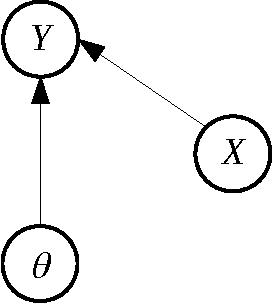
\includegraphics[width=.25\textwidth]{generative.pdf}\label{fig:generative}}
\hspace*{.2\textwidth}
\subfigure[Discriminative model]{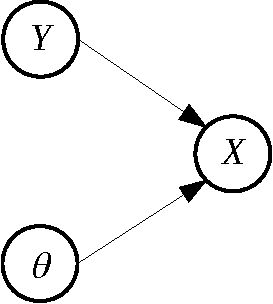
\includegraphics[width=.25\textwidth]{discriminative.pdf}\label{fig:discriminative}}
\caption{Bayesian networks representing generative and discriminative models, where $X$, $Y$ and $\theta$ respectively denote the variable of interest, the data, and the model parameters. Note the marginal independence of~$Y$ and~$\theta$ in the discriminative model.}
\label{fig:graph_comparison}
\end{center}
\end{figure}

Composite likelihood (CL, see \cite{Varin-11} and the references therein) is a semi-generative approach to statistical inference that extends the familiar notion of likelihood without requiring a full generative model. The key idea is to model an arbitrary set of low-dimensional features separately and then combine them, instead of modeling the data distribution as a whole. This may be viewed as a {\em divide and conquer} method to approximate the true but intractable likelihood. While maximum CL does not inherit the general property of maximum likelihood to yield an asymptotically minimum-variance estimator, it is consistent under mild conditions \cite{Xu-11} and may offer an excellent trade-off between computational and statistical efficiency in practice. 

In this note, CL is interpreted as a probabilistic opinion pool of ``agents'' making use of different pieces of information, or clues, extracted from the input data. Each agent acts as an isolated generative model-based statistician and expresses an opinion based on a single clue in the form of a likelihood function of the hidden variables. The agent opinions are then aggregated into a probability distribution on the hidden variables analogous to a Bayesian posterior.

We further argue that a particular log-linear opinion pool yields the best possible predictive distribution in the sense of maximum relative conditional entropy. This perspective entails a method to optimize the weights of the different agents from training data as in a typical discriminative learning scenario. 

%Something for true statisticians. Maybe we could clarify that we use the term ``Bayesian'' in the sense of ``empirical Bayesian'', implying that the parameters $\theta$ are to be estimated somehow contrary to a ``full Bayesian'' approach where they would be integrated out at inference time.


\section{Composite likelihood as opinion pooling}
\label{sec:pool}

Let $Y$ an observable multivariate random variable with sampling distribution $p(y|x)$ conditional on some unobserved variable of interest, $X\in{\cal X}$, where ${\cal X}$ is a known set. Given an experimental outcome $y$, the likelihood is the sampling distribution evaluated at $y$, seen as a function of $x$:
$$
L(x) = p(y|x)
.
$$

This requires a plausible generative model which, for complex data, may be out of reach or involve too many parameters to be estimated. A natural workaround known as {\em data reduction} is to extract some lower-dimensional representation $z=f(y)$, where $f$ is a many-to-one mapping, and consider the potentially more convenient likelihood function:
$$
\ell(x) = p(z|x)
.
$$

Substituting $L(x)$ with $\ell(x)$ boils down to restricting the sample space, thereby  ``delegating'' statistical inference to an ``agent'' provided with partial information. While it is valid for such an agent observing~$z$ only to consider $\ell(x)$ as the likelihood function of the problem, the drawback is that $\ell(x)$ might yield too vague a prediction of~$X$ due to the information loss incurred by data reduction. To make the trick statistically more efficient, we may extract several features, $z_i=f_i(y)$ for $i=1,2,\ldots,n$, and try to combine the likelihood functions $\ell_i(x) = p(z_i|x)$ that they elicit.

If we see the likelihoods as posterior distributions corresponding to uniform priors, this is a classical problem of probabilistic opinion aggregation from possibly redundant sources, for which several methods exist in the literature \cite{Tarantola-82,Genest-86,Garg-04,Allard-12}. We will show in Section~\ref{sec:maxent} that one that is particularly well-suited to our case is the {\em log-linear opinion pool}: 
\begin{equation}
\label{eq:log_pool}
p_\lambda(x|y) = \frac{1}{z_\lambda(y)} \pi(x) \prod_{i=1}^n p(z_i|x)^{\lambda_i},
\end{equation} 
where $\pi(x)$ is some reference distribution or prior, and $\lambda=(\lambda_1,\ldots,\lambda_n)$ is a vector of weights so that the normalizing factor:
$$
z_\lambda(y) = \int \pi(x) \prod_{i=1}^n p(z_i|x)^{\lambda_i} dx
$$
is finite, which holds whenever $\lambda\succeq 0$, {\em i.e.} all weights are positive, assuming that the agent opinions are always upper bounded. Negative weights should be ruled out as the existence condition $z_\lambda(y)<\infty$ would then depend on the particular opinions expressed by the agents. Also note that, while it is possible to have the weights depend on~$y$, there is a strong rational for constant weights as we shall see in the sequel. 

%Strictly positive weights guarantee the so-called 0/1 forcing property, that is, if an hypothesis~$x$ has zero likelihood according to at least one agent, then its consensus probability vanishes too.

% Not clear yet as to what a negative weight could mean!

The log-linear pool~(\ref{eq:log_pool}) bears a striking similarity to Bayes rule, yielding the form: $p_\lambda(x|y)\propto \pi(x) L^c_\lambda(x)$, where the quantity:
\begin{equation}
\label{eq:comp_lik}
L^c_\lambda(x) \equiv \prod_{i=1}^n \ell_i (x)^{\lambda_i}
\end{equation} 
plays the same role as a traditional likelihood function. This expression happens to be known in statistics as a {\em marginal composite likelihood} \cite{Varin-11}. See Appendix~\ref{sec:conditional} for the slightly more general form called {\em conditional composite likelihood}, which can be derived in the same way.

From~(\ref{eq:comp_lik}), we see that CL shares a convenient factorized form with the likelihood derived under the assumption of mutual feature independence, usually referred to as {\em na\"ive Bayes} or {\em simple Bayes} in the machine learning literature, which corresponds to the special case of unitary weights, $\lambda_1=\ldots=\lambda_n= 1$. The clear computational advantage of CL over the true likelihood is that it only requires to evaluate the marginal feature distributions rather than the joint distribution of all features.


\section{Tuning composite likelihood weights}

When the features can be considered exchangeable, it is natural to choose uniform CL weights. The CL is then a scaled version of the na\"ive Bayes likelihood, the common weight value being irrelevant to the maximum CL estimator (MCLE). The weight may be tuned so as to best adjust the pseudo posterior variance matrix to the asymptotic variance matrix of the MCLE \cite{Pauli-11}, or via a close-in-spirit curvature adjustment \cite{Ribatet-12}, in attempts to match the frequentist and composite Bayesian notions of uncertainty.

Ignoring such a goal, another frequent recommandation for CL weights is to sum up to one. This can be motivated in various ways. It turns out that the only pooling operator that does not explicitly depend on~$x$ and preserves {\em external Bayesianity} is the log-linear opinion pool with unit sum weights \cite{Genest-86b}. External Bayesianity essentially means that it should not matter whether the prior is incorporated before or after pooling, provided that all agents agree on the same prior. Another appealing property of log-linear pooling with unit sum weights is to minimize the average Kullback-Leibler (KL) divergence to the agent opinions \cite{Garg-04}. A maximum relative entropy property is also given in \cite{Wang-14}, Theorem~3.

Unit sum weights, however, correspond to the extreme situation where the features are assumed to be maximally redundant, but is clearly ineffective for independent or weakly correlated features, which require weights close to one for the CL to closely approximate the true likelihood. In this case, the CL may be much flatter than it should, leading to severly overestimated credibility sets.

{\color{red} Why is it important to fine-tune the weights?}
We therefore need a method to tune weights that can automatically adjust to the level of statistical dependence beween features.

%Instead, redundancy between agents is assumed by default, and is effectively encoded by the unit sum constraint on weights\footnote{Nevertheless, features which are {\em known} to be mutually independent can be merged into a single feature. This results in increasing their weights in the log-linear pool.}.

\section{Maxent composite likelihood}
\label{sec:maxent}

We can derive composite likelihood from the conditional maximum entropy principle \cite{BergerA-96}. It comes with a method of tuning weights, hence a particular composite likelihood function that we call maxent composite likelihood (MCL).

A cheap MaxEnt argument was already given by \cite{Wang-14}  (standard, non-conditional MaxEnt at fixed $y$, hence just an existence result but no feasible weight tuning).

What we do here is maximum {\em conditional} entropy. It's slightly more complex than a simple $I$-projection. The search space is a set of predictive distributions compatible with mean log-likelihood contraints. If I know the generative distribution, I know the expected log-likelihood.

We work with inequality constraints to force $\lambda\geq 0$:
$$
E[\log p(z_i|x)] \geq c_i \equiv \int \pi(x)p(z_i|x) \log p(z_i|x) dx dy
$$

What does the constraint mean? It means that a model is admissible if it compresses the data at least as well as all my agents. So we are not assuming that the generative models are {\em true}. We only assume that they are useful to compress the (reduced) data. Connection to MDL. 

Why not using the feature-based posteriors or Bayes factors rather than the likelihoods? It's a possibility (perhaps a connection here with Gr\"unwald's luckiness). A justification for not doing it is that the coordinator should discard the priors used by the agents. The constraints are not purely evidence-based since the moments depend on the coordinator's prior but it is arguable a mess of priors wouldn't be good.

Intuition behind weights: Lagrange multipliers to enforce a constraint... Notion of feature relevance. But does $\lambda_1>\lambda_2$ imply that $z_1$ is more relevant than $z_2$? 

The derivation assumed the marginal distribution of the data $h(y)$ to be known. In practice, it is estimated by the empirical distribution just like the moments are estimated.

Game theoretic interpretation \cite{Grunwald-04}.

The dual function boils down to the famous cross-entropy.

Single feature case ($y=z$): the maxent solution has the form $p(x|y)\propto\pi(x)p(y|x)^\lambda$. We expect to have $\lambda=1$ but it's not necessarily the case. It is if $h(y)=\int\pi(x)p(y|x)dx$ because then $h(y)p(x|y)=\pi(x)p(y|x)$ so the constraint is verified (and active). This also tells us that the data marginal should be consistent with the prior on labels for this much expected consistency property to hold. So, either weight datapoints so as to match a desired prior (e.g., uniform) or take the empirical distribution of labels as the ``prior''. 

Which brings another question: in this case, the (unique) weight is insensitive to the prior -- is it true in general? The answer is no. The weights generally depend on the prior. Hence the maxent composite likelihood is prior-dependent. This is an important conceptual difference with the classical notion of likelihood.

\section{Super composite likelihood}
\label{sec:super}

When chosen for computational simplicity, clues may not only convey limited information at individual level: their informativeness may also be very much hypothesis-dependent. Consider, for instance, diagnosing a disease from a routine medical checkup. Body temperature may point to a bacterial infection by comparison with normality, but would not help detecting a non-infectious cardiovascular disease -- and conversely for, say, blood pressure.

This motivates a more general setting where clues can be weighted differently depending on hypotheses.

What happens if we use mean-values constraints conditional on $x$ instead of jointly averaged over $x$ and $y$? This boils down to picking functions of the form:
$$
\chi(x-a)\ell_i(x,y)
$$

The answer is that the maxent solution has the form:
$$
p_\lambda(x|y) = \pi(x) \prod_i p(z_i|x)^{\lambda_i(x)}
$$

In other words, the weights become dependent on the variable of interest. This is the super composite likelihood idea.


\section{Composite EM algorithm for unsupervised learning}
\label{sec:gem}

In a nutshell: alternate unsupervised learning of partial model parameters ($M$-step) and re-estimation of label posteriors via maxent ($E$-step). 

$M$-step: given a posterior estimate $q(x|y)$, do just as if the features were independent and solve: 
$$
\max_\theta
\int \sum_i h(y)q(x|y) \log p_\theta(z_i,x) dx dy
$$

Note we can estimate cross-feature parameters such as class proportions.

Surrogate $E$-step: given generative parameters, recompute the moment constraints and update $q(x|y)$ according to the conditional maxent principle:
$$
\min_q
\int h(y)q(x|y) \log \frac{q(x|y)}{\pi(x)} dx dy
$$
s.t.
$$
\int h(y)q(x|y)\log p_\theta(z_i|x) dx dy \geq \int \pi(x)p_\theta(z_i|x)\log p_\theta(z_i|x) dx dy
$$

However, there is an important issue: how is $h(y)$ defined in both the $M$- and $E$-steps? In supervised context, $h(x,y)$ can be defined beforehand as the prior-corrected empirical distribution:
$$
h(x,y) = \pi(x) \frac{h_0(x,y)}{h_0(x)},
$$
where $h_0(x,y)$ is the raw empirical distribution. In unsupervised context, the best we can do is to replace $h_0(x,y)$ with $h_0(y)q(x|y)$, implying that the empirical distribution of $y$ is reweighted according to:
$$
h(y) = \sum_i w_i\delta(y-y_i),
\qquad
w_i = \int \pi(x)\frac{q(x|y_i)}{\sum_j q(x|y_j)} dx,
$$
which needs to be done each time $q(x|y)$ is updated, that is, after each $E$-step.

The other option is to keep $h(y)$ constant throughout the iterations but adapt $\pi(x)$ as the marginal distribution of labels learned in the $M$-step. In this case, it's no longer a ``prior''. 

Are we minimizing a unique functional as in the variational EM algorithm? Possibly not. We may see this generalization as a two-player game. One player tries to predict several data features independently. The other player tries to predict labels. Together, they find patterns (clusters) in unlabeled data. Does the more general version converge? Does the game have a value? And so on.

In the case of a single feature, is this the well-known EM? The $M$-step is clearly the same, what about the $E$-step? It is the same if $h(y)p_\theta(x|y)=p_\theta(y|x)\pi(x)$. However, this condition won't hold if $h(y)$ is an empirical distribution... In this special case, the ``E player'' could use the data distribution model produced by the ``M player'' instead of the empirical one but, more generally, there is no data distribution model so he has to stick to the empirical one.

The maxent is a surrogate for the $E$-step. It reflects the lack of a full model $p_\theta(x,y)$.

% Accounting here for Xi'An comment on xianblog.wordpress.com
% The sum of the powers is constrained to be equal to one, even though
% I do not understand why the dimensions of the projections play nog
% role in this constraint. Simplicity is advanced as an argument,
% which sounds rather weak…
%This simple constraint is implied by the external Bayesianity requirement: as it turns out, the only aggregation operator which is both externally Bayesian and independent from $x$ boils down to plugging a composite likelihood with unit sum weights into Bayes rule, hence extending the classical notion of likelihood in Bayesian analysis.


\section{Discussion}
\label{sec:discussion}

Deep learning is discriminative...

CL is a concept from computational statistics that has mainly been developed so far in a frequentist perspective as a surrogate for the maximum likelihood method. We have shown a deep connection between CL and probabilistic inference, thereby establishing CL as a class of discriminative models. Because CL is built from a set of marginal feature-specific generative distributions, it is in essence a two-step semi-generative, semi-discriminative learning approach. In the first, ``generative'' phase, the feature distributions are learned; in the second, ``discriminative'' phase, the feature weights are learned. This strategy can be thought of as a form of non-adaptive boosting.

%The first phase corresponds to the training of ``weak learners''. The second phase amounts to a form of boosting. 

A purely discriminative learning could be used instead but...
Why potentially more efficient than pure discriminative training: because generative training is always more efficient than discriminative training if models are comparable. So the key point is that ``we have less parameters in the discriminant phase". Good in small datasets. But also in asymptotic regime if the features are weakly or highly correlated (???).

Logistic regression / naive Bayes example. Under homoscedasticity (assuming that each feature has class-independent variance), CBI is equivalent to logistic regression -- because the predictive distribution family is the same. This is a case where BCI brings nothing. But consider heteroscedasticity, then BCI yields a quadratic classifier. Compared to a fully discriminative model, the number of parameters to learned in the discriminative phase is reduced by half.

The first training phase is easier if supervised but could be unsupervised too (using mixture models). How do we then deal with label switching issues? Can we safely assume conditional feature independence {\em in the generative training phase}? I believe so provided that the marginal distribution parameters are disjoint. It's obvious in the supervised learning scenario.

If unsupervised, the first learning phase could be compared with contrastive pre-training of RBMs \cite{Hinton-06,Fischer-14}, which also optimize parameters for generation of observable features. BCI is comparable with an RBM with a single output unit (which is just a generative model assuming conditionial feature independence). The key difference is that the RBM is a full generative model while BCI only deals with marginal models, hence relying on weaker assumptions. This won't change anything in the pre-training phase but RBMs have to deal with more parameters in the generative learning phase. In fully supervised context, RBM pre-training is pointless since all parameters learned in the first phase will be overwritten. In BCI, pre-training is crucial even in supervised context because the parameters learned in the discriminative phase (the feature weighs) describe a sub-manifold of the predictive distribution family.

Needs features. Not a representation learning method, but could be coupled why not.


%{\color{red} Moreover, while RBM parameters are typically refined in a supervised discriminative learning step, disjoint set of parameters for SCL. Dunno how to say that.} 

%In such context, SCL competes with classical discriminative models (logistic regression, Gaussian processes \cite{Rasmussen-06}, maximum entropy models \cite{BergerA-96}, etc.), and may compare more or less favorably in practice depending on the amount of training data. For relatively small training datasets, we may hope for more accurate inference using~SCL than using traditional discriminative models, extrapolating from the results of \cite{Ng-01} regarding the comparison between logistic regression and na\"ive Bayes classifiers.
%{\color{red}Ici, il manque la comparaison avec les RBMs qui ne sont pas (forcement) des modeles discriminatifs.}

%%, hence alleviating the need for heavily supervised model training

%In summary, CL has the potential to yield weakly supervised or unsupervised Bayesian-like inference procedures depending on the particular task at hand. This property reflects the encoding of statistical relationships between the data and {\em all} unknown parameters. CL thus appears as a trade-off between generative models, which are optimal for unsupervised learning but possibly intractable, and traditional discriminative models (logistic regression, Gaussian processes \cite{Rasmussen-06}, maximum entropy models \cite{BergerA-96}, etc.), which are inherently supervised. CL models are discriminative models assembled from atomic generative models and, from this point of view, may be considered as {\em semi-generative} models.

%CL may be considered as a {\em semi-generative} model: a discriminative model assembled from partial generative models.

%As a note of caution, we shall stress that the pre-determined weights assigned to the different associations between observed and unobserved values represent prior knowledge regarding the informativeness of clues. A poor choice of weights will inevitably result in a poor approximation to the ``true'' Bayesian posterior -- the posterior that would be obtained from a realistic generative model if it was tractable. In future work, we will investigate feature selection strategies to mitigate this problem.

% Improve the discussion on following aspects:
% ** Why is it compatible with unsupervised learning? Give more insight.
% ** Stress the contribution: class-specific weighting.
% * Pivotality argument.
% * Bayes is a special case of composite Bayes.

{\color{red}Product of fucking experts \cite{Hinton-02}. Log-linear pool to build a generative model (assuming in fact independence between experts). Better seen as a ``log-mixture model''. Sounds like each expert is associated with a class, so it's the same as a RBM. Contrastive learning approximates ML parameter estimation. The experts are learning jointly. It's just a generative model.}

{\color{red}Two-step training: generative phase then discriminative phase. Why is it cool?}

{\color{red}CBI is just a way to reweight Naive Bayes. What's the big deal? Can we really expect massively superior performance? Are we just talking about realistic credibility sets?}


\appendix

\section{Conditional composite likelihood}
\label{sec:conditional}

As a straightforward  extension of marginal CL, each feature-based likelihood may be conditioned by an additional ``independent'' feature $z^c_i = f^c_i(y)$ considered as a predictor of the ``dependent'' feature, $z_i=f_i(y)$, yielding the more general form:
\begin{equation}
\label{eq:cond_feat_lik}
\ell_i(x) = p(z_i|x,z^c_i).
\end{equation}

Conditioning may be useful if it is believed that $z^c_i$ alone is little or not informative about $x$, but can provide relevant information when considered jointly with $x$, as in the case of regression covariates, for instance. Equation~(\ref{eq:comp_lik}) then amounts to conditional CL \cite{Varin-11}, a more general form of CL also including Besag's historical {\em pseudo-likelihood} \cite{Besag-74} developed for image segmentation.


\section{Minimally discriminative model}

Let $\pi(x)$ some reference distribution that represents full
uncertainty about $X$. We wish to select the joint distribution
$p(x,y)$ that minimizes:
$$
I(p) = \int p(x,y) \log \frac{p(x|y)}{\pi(x)} dy,
$$ subject to feature mean-value constraints of the form:
$$
\int p(x,y) f(x,y) dx dy = \mu.
$$

There are two special cases of this problem in the literature.  On the
one hand, the {\em maximum entropy classifier} \cite{BergerA-96}
incorporates the constraint that $p(y)$ be known, however we will see
that this is not necessary. The {\em minimally informative likelihood}
method \cite{Yuan-99b,Yuan-99}, on the other hand, imposes that
$p(x)=\pi(x)$, hence assuming the form $p(x,y)=\pi(x)p(y|x)$. We won't
make such assumptions here and will consider the case where $\mu$ is
completely unknown.

The above problem is seen to be equivalent to minimizing the auxiliary
objective function:
$$
I(p,m) 
= \int p(x,y) \log \frac{p(x,y)}{\pi(x)m(y)} dxdy,
$$ over $p$ and $m$, subject to the same constraints on $p$. We note
that $I(p,m)=I(p)+D(p_y\|m)$, showing that the auxiliary function
essentially adds a penalty term to the actual objective in order to
force $p(y)$ close to $m(y)$.

Minimizing $I(p,m)$ along both $p$ and $m$ is basically a minimum KL
divergence problem between two convex distribution spaces, so there
must be a unique solution {\bf -- to be checked in
  \cite{Cover-91}}. It is similar to the rate-distortion problem in
information theory, which may be solved by alternate minimization,
yielding a Blahut-Arimoto algorithm.
\begin{itemize}
\item {\em Let's call it A-step}. Optimize $p(x,y)$ at fixed $m$
  s.t. constraint:
$$
\exists \lambda, \qquad
p_{\lambda,m}(x,y) = \frac{1}{Z(\lambda, m)} \pi(x) m(y) e^{-\lambda^\top t(x,y)}
$$
The actual $\lambda$ is found my maximizing the dual function
$\psi(\lambda,m)$, see below.
\item {\em Let's call it B-step}. Optimize $m(y)$ at fixed $p(x,y)$:
$$
m(y) = \int p(x,y) dx
$$
\end{itemize}

Upon convergence, the algorithm outputs both joint and marginal
distributions $p_{\star}(x,y)$ and $m_{\star}(y)$ that both depend on
$\mu$. By construction, we have that $p_{\star}(y) = m_{\star}(y)$,
therefore $p_\star(x|y)=p_{\star}(x,y)/m_{\star}(y)$.


\section{Comparison with maximum entropy classifier}

Lagrangian...
$$
{\cal L}(p,m,\lambda)
= 
\int p(x,y) \log \frac{p(x,y)}{\pi(x)m(y)} dxdy
+
\lambda^\top \left( 
\int p(x,y) f(x,y) dydy - \mu 
\right)
$$ where $\lambda$ represents a vector-valued Lagrange multiplier. At
fixed $m$, the solution has the form:
$$
p_{\lambda,m}(x,y) = \frac{1}{Z(\lambda,m)}
\pi(x) m(y) e^{-\lambda^\top f(x,y)} 
$$

Note that this implies that the conditional distribution is
independent of $m$ once $\lambda$ is determined,
$$
p_\lambda(x|y) = \frac{1}{z(\lambda,y)} \pi(x) e^{-\lambda^\top f(x,y)} 
$$

Also, the marginal is a modulation of $m(y)$:
$$
p_{\lambda,m}(y) = \frac{z(\lambda,y)}{Z(\lambda,m)} m(y)
$$

Dual function at fixed $m$:
$$
\psi(\lambda,m) 
\equiv \min_p {\cal L}(p,m,\lambda)
= 
- \log Z(\lambda,m) - \lambda^\top \mu
.
$$ 

An alternative expression is:
$$
\psi(\lambda, m)
= 
\int h(x,y) 
\log \frac{p_{\lambda,m}(x,y)}{\pi(x)m(y)} dxdy,
$$ where $h(x,y)$ is any distribution statisfying the
constraints. This shows that maximizing the dual function at fixed $m$
is essentially the same as minimizing the KL divergence
$D(h\|p_{\lambda,m})$ over $\lambda$, in other words fitting $h(x,y)$
by some distribution of the form $p_{\lambda,m}$. The fact that the
result does not depend on the particular $h(x,y)$ that is chosen, as
long as it satifies the constraint, is a general property of
exponential families.

We also have that the dual function associated with $I(p)$ reads:
\begin{eqnarray*}
\psi(\lambda) 
 & = & \min_m \psi(\lambda, m)\\
 & = & \int h(x,y) \log \frac{p_{\lambda}(x|y)}{\pi(x)} dxdy\\
 & = & -\int h(y) \log z(\lambda,y) dy - \lambda^\top \mu
\end{eqnarray*}

But, wait, that's exactly what we get in the maximum entropy
classifier! So, at the end of the day, we simply got an alternative
method to learn $\lambda$ in the maximum entropy classifier, i.e. the
Blahut-Arimoto algorithm as opposed to a brute-force maximization of
$\psi(\lambda)$. Both methods will converge to the same $\lambda$...

What it essentially means is that the optimal $\lambda$ is insensitive
to $m(y)$ as long as $m(y)$ is compliant in the sense that:
$$
m(y) = \int h(x,y) dx,
$$ for some distribution $h(x,y)$ statisfying the constraint. This is
true for the optimal $m_\star(y)$ output by the BA algorithm, but
also, for instance, for the empirical distribution of observations in
a training dataset used to estimate $\mu$, as proposed in
\cite{BergerA-96}. The only special property of $m_\star(y)$ is to
yield the full Bayesian model $p_\star(x,y)=p_\star(x|y)m_\star(y)$
that minimizes the discrimination information. We may not care too
much about that in practice since we will only use $p_\star(x|y)$. 

\section{Comparison with minimally informative likelihood}

Yuan \cite{Yuan-99} considered the situation where we add the
constraint that $p(x)=\pi(x)$ to the minimum discrimination inference
problem. Unknown is then the conditional distribution
$p(y|x)$. Lagrangian...
\begin{eqnarray*}
{\cal L}(p,m,\lambda)
 & = & 
\int \pi(x)p(y|x) \log \frac{p(y|x)}{m(y)} dxdy
+
\lambda^\top \left( 
\int \pi(x)p(y|x) f(x,y) dydy - \mu 
\right) \\
 & = & 
\int \pi(x)
\left( 
\int
p(y|x) \log \frac{p(y|x)}{m(y)} dy
+
\lambda^\top 
\int p(y|x) f(x,y) dy
- \mu 
\right)
dx 
\end{eqnarray*}

The derivative is given by,
$$
\frac{\partial\cal L}{\partial p(y|x)}
= 
\pi(x)\left[ 
1 + \log \frac{p(y|x)}{m(y)} 
+ \lambda^\top f(x,y)
\right],
$$
hence the optimal model at fixed $m$ has the form:
$$
p_{\lambda,m}(y|x) = \frac{1}{Z(\lambda,m,x)} m(y) e^{-\lambda^\top f(x,y)} 
$$

Note that the induced posterior distribution $p_{\lambda,m}(x|y)$ has
a different form from above unless the normalizing factor
$Z(\lambda,m,x)$ turns out independent from $x$. If this is not the
case, we no longer have the property that $p_{\lambda,m}(x|y)$ is
independent from $m$ given $\lambda$.

Dual function...
$$
\psi(\lambda,m) 
=
- \int \pi(x) \log Z(\lambda, m, x) dx
- \lambda^\top \mu
$$

Equivalently, for any distribution under the form $\pi(x)h(y|x)$ that
satisfies the moment constraint, we have:
$$
\psi(\lambda,m) 
=
\int \pi(x) h(y|x) \log \frac{p_{\lambda,m}(y|x)}{m(y)} dxdy
$$

Now, the real question is why should we constrain $p(x)$, which boils
down to a Bayesian prior in this context, to be the same as our
reference $\pi(x)$? It only makes sense if we want our inference to
stick to a generative modeling paradigm... but haven't we already
given up on that? Therefore, unless we find a good reason not to, we
won't impose the $p(x)=\pi(x)$ constraint, thereby allowing for a
discrepancy between the reference and the prior.


\section{Discriminative vs. semi-discriminative}

Let's go back to the equivalence we found between our approach and the
maximum entropy classifier (MCE) \cite{BergerA-96}. We have said that
the former is essentially a re-formulation of MCE.

But the re-formulation also conveys a generalization of MCE if,
instead of letting $m$ being an arbitrary distribution, we restrict
its search space to some set of acceptable reference
distributions. Would such a strategy be useful? 

Recall that the method selects the joint distribution that minimizes
discriminative information, as defined by $I(p)$:
$$
I(p) 
= \int p(x,y)\log\frac{p(x|y)}{\pi(x)} dxdy
= E_Y[D(p_{x|y}\|\pi)]
$$

The latter characterization reminds us that discriminative information
is defined in an average sense. The corresponding posterior $p(x|y)$
may not be conservative for some $y$, in particular those that are
unlikely under $p(y)$. It would be a problem if that's the case for
the particular data at hand. For that to happen rarely, the ideal
$p(y)$ would be the ``true'' marginal distribution of $Y$.

However, for vague mean value constraints, nothing may prevent the
optimal $m_\star(y)$ from departing significantly from that ideal
distribution. In fact, we can show that $m_\star(y)$ only has mass at
$y$ values that maximize $z(\lambda_\star,y)$, and is therefore likely
sparse. This is because $m_\star$ minimizes $\psi(\lambda_\star,m)$,
which is equivalent to maximizing $Z(\lambda_\star,m)$ and we have:
$$
Z(\lambda, m) = \int m(y) z(\lambda, y) dy.
$$

In other words, the solution to our problem may be singular! It does
not hurt since, as discussed above, one may alternatively fix $m(y)$
to some pre-defined distribution... but this, in practice, restricts
the method to supervised learning situations.

We may not face this issue with the MIL method, which further imposes
the prior on $X$, so all the information from the constraints goes
into specifying a possibly reasonable generative model.



\bibliographystyle{abbrv}
\bibliography{cvis,stat,alexis}

%%\documentclass[english]{scrartcl}

\usepackage{fullpage}
\usepackage{amstext,amssymb,amsmath,amsthm}
\usepackage{graphicx,subfigure}
\usepackage{multirow}
\usepackage{url}
\usepackage{hyperref}
\usepackage{color}

\graphicspath{{.}{pics/}}

%\newtheorem{theorem}{Theorem}[section]
%\newtheorem{proposition}[theorem]{Proposition}


\title{Composite Bayesian inference}
\date{}
\author{Alexis Roche\thanks{\url{alexis.roche@centraliens.net}}}

%\newcommand{\fix}{\marginpar{FIX}}
%\newcommand{\new}{\marginpar{NEW}}
%\newcommand{\matphi}{\boldsymbol{\Phi}} 
%\def\x{{\mathbf{x}}}
%\def\z{{\mathbf{z}}}
%\def\u{{\mathbf{u}}}
%\def\p{{\bar{\mathbf{p}}}}
%\def\q{{\bar{\mathbf{q}}}}



\begin{document}

\maketitle

\begin{abstract}
This note revisits the concept of composite likelihood from the perspective of probabilistic inference, and advocates a machine learning approach to tune the associated ``weights'', which stems naturally from a connection with the maximum entropy principle: the predictive distribution that maximizes conditional entropy relative to a given prior and subject to multiple mean log-likelihood inequality constraints is, up to a normalizing factor, the prior multiplied by a particular composite likelihood function, hence providing a ``composite'' extension of Bayes rule. We argue that composite Bayesian inference is a middle way between generative and discriminative approaches to statistical inference, which can be powerful in shallow learning and transfer learning problems.
\end{abstract}


\section{Introduction}
\label{sec:intro}

Classical frequentist and Bayesian inference paradigms rest upon the existence of a probabilistic data-generating model that is both empirically valid and computationally tractable. Because this is challenging for complex data, other inference models are commonly used in applied science: deliberately misspecified generative models, as in quasi-likelihood methods \cite{White-82,Walker-13} or na\"ive Bayes \cite{Ng-01}; data compression models as in minimum description length \cite{Grunwald-07}; and discriminative models\footnote{A {\em discriminative} model is a parametric family that describes the distribution of a variable of interest conditional on data, in contrast with a {\em generative} model, which describes the conditional distribution of data given the variable of interest.}, which currently dominate the field of artificial intelligence and typically require massive supervised learning -- these include classical techniques (maximum entropy classifiers \cite{BergerA-96}, support vector machines \cite{Vapnik-00}, Gaussian processes \cite{Rasmussen-06}) as well as most deep learning techniques \cite{Lecun-15,Goodfellow-16} with the exception of deep belief networks \cite{Hinton-06,Fischer-14}. 

A strong limitation of discriminative models is that they are not suitable for unsupervised learning or on-the-fly parameter estimation because they treat the data and the model parameters as {\em marginally independent}, meaning that the data conveys no information about the parameters unless the variable of interest is observed. This is illustrated in Figure~\ref{fig:graph_comparison} by the respective directed graph representations of generative and discriminative models. For the same reason, supervised learning in a discriminative model is less precise than in a generative model spanning the same family of posteriors, hence it is less effective in small training sets \cite{Ng-01}. Overall, pure discriminative models are of little use outside the context of big labeled data.

% p(x,y|theta) = p(x|y,theta)p(y|theta)

\begin{figure}[!ht]
\begin{center}
\subfigure[Generative model]{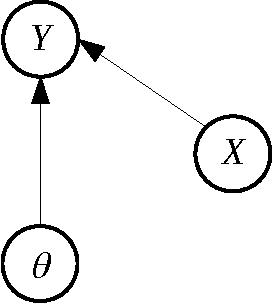
\includegraphics[width=.25\textwidth]{generative.pdf}\label{fig:generative}}
\hspace*{.2\textwidth}
\subfigure[Discriminative model]{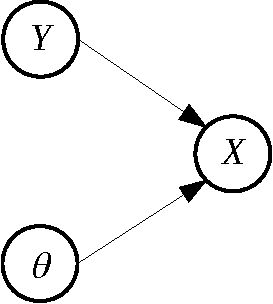
\includegraphics[width=.25\textwidth]{discriminative.pdf}\label{fig:discriminative}}
\caption{Bayesian networks representing generative and discriminative models, where $X$, $Y$ and $\theta$ respectively denote the variable of interest, the data, and the model parameters. Note the marginal independence of~$Y$ and~$\theta$ in the discriminative model.}
\label{fig:graph_comparison}
\end{center}
\end{figure}

Composite likelihood (CL, see \cite{Varin-11} and the references therein) is a semi-generative approach to statistical inference that extends the familiar notion of likelihood without requiring a full generative model. The key idea is to model an arbitrary set of low-dimensional features separately and then combine them, instead of modeling the data distribution as a whole. This may be viewed as a {\em divide and conquer} method to approximate the true but intractable likelihood. While maximum CL does not inherit the general property of maximum likelihood to yield an asymptotically minimum-variance estimator, it is consistent under mild conditions \cite{Xu-11} and may offer an excellent trade-off between computational and statistical efficiency in practice. 

In this note, CL is interpreted as a probabilistic opinion pool of ``agents'' making use of different pieces of information, or clues, extracted from the input data. Each agent acts as an isolated generative model-based statistician and expresses an opinion based on a single clue in the form of a likelihood function of the hidden variables. The agent opinions are then aggregated into a probability distribution on the hidden variables analogous to a Bayesian posterior.

We further argue that a particular log-linear opinion pool yields the best possible predictive distribution in the sense of maximum relative conditional entropy. This perspective entails a method to optimize the weights of the different agents from training data as in a typical discriminative learning scenario. 

%Something for true statisticians. Maybe we could clarify that we use the term ``Bayesian'' in the sense of ``empirical Bayesian'', implying that the parameters $\theta$ are to be estimated somehow contrary to a ``full Bayesian'' approach where they would be integrated out at inference time.


\section{Composite likelihood as opinion pooling}
\label{sec:pool}

Let $Y$ an observable multivariate random variable with sampling distribution $p(y|x)$ conditional on some unobserved variable of interest, $X\in{\cal X}$, where ${\cal X}$ is a known set. Given an experimental outcome $y$, the likelihood is the sampling distribution evaluated at $y$, seen as a function of $x$:
$$
L(x) = p(y|x)
.
$$

This requires a plausible generative model which, for complex data, may be out of reach or involve too many parameters to be estimated. A natural workaround known as {\em data reduction} is to extract some lower-dimensional representation $z=f(y)$, where $f$ is a many-to-one mapping, and consider the potentially more convenient likelihood function:
$$
\ell(x) = p(z|x)
.
$$

Substituting $L(x)$ with $\ell(x)$ boils down to restricting the sample space, thereby  ``delegating'' statistical inference to an ``agent'' provided with partial information. While it is valid for such an agent observing~$z$ only to consider $\ell(x)$ as the likelihood function of the problem, the drawback is that $\ell(x)$ might yield too vague a prediction of~$X$ due to the information loss incurred by data reduction. To make the trick statistically more efficient, we may extract several features, $z_i=f_i(y)$ for $i=1,2,\ldots,n$, and try to combine the likelihood functions $\ell_i(x) = p(z_i|x)$ that they elicit.

If we see the likelihoods as posterior distributions corresponding to uniform priors, this is a classical problem of probabilistic opinion aggregation from possibly redundant sources, for which several methods exist in the literature \cite{Tarantola-82,Genest-86,Garg-04,Allard-12}. We will show in Section~\ref{sec:maxent} that one that is particularly well-suited to our case is the {\em log-linear opinion pool}: 
\begin{equation}
\label{eq:log_pool}
p_\lambda(x|y) = \frac{1}{z_\lambda(y)} \pi(x) \prod_{i=1}^n p(z_i|x)^{\lambda_i},
\end{equation} 
where $\pi(x)$ is some reference distribution or prior, and $\lambda=(\lambda_1,\ldots,\lambda_n)$ is a vector of weights so that the normalizing factor:
$$
z_\lambda(y) = \int \pi(x) \prod_{i=1}^n p(z_i|x)^{\lambda_i} dx
$$
is finite, which holds whenever $\lambda\succeq 0$, {\em i.e.} all weights are positive, assuming that the agent opinions are always upper bounded. Negative weights should be ruled out as the existence condition $z_\lambda(y)<\infty$ would then depend on the particular opinions expressed by the agents. Also note that, while it is possible to have the weights depend on~$y$, there is a strong rational for constant weights as we shall see in the sequel. 

%Strictly positive weights guarantee the so-called 0/1 forcing property, that is, if an hypothesis~$x$ has zero likelihood according to at least one agent, then its consensus probability vanishes too.

% Not clear yet as to what a negative weight could mean!

The log-linear pool~(\ref{eq:log_pool}) bears a striking similarity to Bayes rule, yielding the form: $p_\lambda(x|y)\propto \pi(x) L^c_\lambda(x)$, where the quantity:
\begin{equation}
\label{eq:comp_lik}
L^c_\lambda(x) \equiv \prod_{i=1}^n \ell_i (x)^{\lambda_i}
\end{equation} 
plays the same role as a traditional likelihood function. This expression happens to be known in statistics as a {\em marginal composite likelihood} \cite{Varin-11}. See Appendix~\ref{sec:conditional} for the slightly more general form called {\em conditional composite likelihood}, which can be derived in the same way.

From~(\ref{eq:comp_lik}), we see that CL shares a convenient factorized form with the likelihood derived under the assumption of mutual feature independence, usually referred to as {\em na\"ive Bayes} or {\em simple Bayes} in the machine learning literature, which corresponds to the special case of unitary weights, $\lambda_1=\ldots=\lambda_n= 1$. The clear computational advantage of CL over the true likelihood is that it only requires to evaluate the marginal feature distributions rather than the joint distribution of all features.


\section{Tuning composite likelihood weights}

When the features can be considered exchangeable, it is natural to choose uniform CL weights. The CL is then a scaled version of the na\"ive Bayes likelihood, the common weight value being irrelevant to the maximum CL estimator (MCLE). The weight may be tuned so as to best adjust the pseudo posterior variance matrix to the asymptotic variance matrix of the MCLE \cite{Pauli-11}, or via a close-in-spirit curvature adjustment \cite{Ribatet-12}, in attempts to match the frequentist and composite Bayesian notions of uncertainty.

Ignoring such a goal, another frequent recommandation for CL weights is to sum up to one. This can be motivated in various ways. It turns out that the only pooling operator that does not explicitly depend on~$x$ and preserves {\em external Bayesianity} is the log-linear opinion pool with unit sum weights \cite{Genest-86b}. External Bayesianity essentially means that it should not matter whether the prior is incorporated before or after pooling, provided that all agents agree on the same prior. Another appealing property of log-linear pooling with unit sum weights is to minimize the average Kullback-Leibler (KL) divergence to the agent opinions \cite{Garg-04}. A maximum relative entropy property is also given in \cite{Wang-14}, Theorem~3.

Unit sum weights, however, correspond to the extreme situation where the features are assumed to be maximally redundant, but is clearly ineffective for independent or weakly correlated features, which require weights close to one for the CL to closely approximate the true likelihood. In this case, the CL may be much flatter than it should, leading to severly overestimated credibility sets.

{\color{red} Why is it important to fine-tune the weights?}
We therefore need a method to tune weights that can automatically adjust to the level of statistical dependence beween features.

%Instead, redundancy between agents is assumed by default, and is effectively encoded by the unit sum constraint on weights\footnote{Nevertheless, features which are {\em known} to be mutually independent can be merged into a single feature. This results in increasing their weights in the log-linear pool.}.

\section{Maxent composite likelihood}
\label{sec:maxent}

We can derive composite likelihood from the conditional maximum entropy principle \cite{BergerA-96}. It comes with a method of tuning weights, hence a particular composite likelihood function that we call maxent composite likelihood (MCL).

A cheap MaxEnt argument was already given by \cite{Wang-14}  (standard, non-conditional MaxEnt at fixed $y$, hence just an existence result but no feasible weight tuning).

What we do here is maximum {\em conditional} entropy. It's slightly more complex than a simple $I$-projection. The search space is a set of predictive distributions compatible with mean log-likelihood contraints. If I know the generative distribution, I know the expected log-likelihood.

We work with inequality constraints to force $\lambda\geq 0$:
$$
E[\log p(z_i|x)] \geq c_i \equiv \int \pi(x)p(z_i|x) \log p(z_i|x) dx dy
$$

What does the constraint mean? It means that a model is admissible if it compresses the data at least as well as all my agents. So we are not assuming that the generative models are {\em true}. We only assume that they are useful to compress the (reduced) data. Connection to MDL. 

Why not using the feature-based posteriors or Bayes factors rather than the likelihoods? It's a possibility (perhaps a connection here with Gr\"unwald's luckiness). A justification for not doing it is that the coordinator should discard the priors used by the agents. The constraints are not purely evidence-based since the moments depend on the coordinator's prior but it is arguable a mess of priors wouldn't be good.

Intuition behind weights: Lagrange multipliers to enforce a constraint... Notion of feature relevance. But does $\lambda_1>\lambda_2$ imply that $z_1$ is more relevant than $z_2$? 

The derivation assumed the marginal distribution of the data $h(y)$ to be known. In practice, it is estimated by the empirical distribution just like the moments are estimated.

Game theoretic interpretation \cite{Grunwald-04}.

The dual function boils down to the famous cross-entropy.

Single feature case ($y=z$): the maxent solution has the form $p(x|y)\propto\pi(x)p(y|x)^\lambda$. We expect to have $\lambda=1$ but it's not necessarily the case. It is if $h(y)=\int\pi(x)p(y|x)dx$ because then $h(y)p(x|y)=\pi(x)p(y|x)$ so the constraint is verified (and active). This also tells us that the data marginal should be consistent with the prior on labels for this much expected consistency property to hold. So, either weight datapoints so as to match a desired prior (e.g., uniform) or take the empirical distribution of labels as the ``prior''. 

Which brings another question: in this case, the (unique) weight is insensitive to the prior -- is it true in general? The answer is no. The weights generally depend on the prior. Hence the maxent composite likelihood is prior-dependent. This is an important conceptual difference with the classical notion of likelihood.

\section{Super composite likelihood}
\label{sec:super}

When chosen for computational simplicity, clues may not only convey limited information at individual level: their informativeness may also be very much hypothesis-dependent. Consider, for instance, diagnosing a disease from a routine medical checkup. Body temperature may point to a bacterial infection by comparison with normality, but would not help detecting a non-infectious cardiovascular disease -- and conversely for, say, blood pressure.

This motivates a more general setting where clues can be weighted differently depending on hypotheses.

What happens if we use mean-values constraints conditional on $x$ instead of jointly averaged over $x$ and $y$? This boils down to picking functions of the form:
$$
\chi(x-a)\ell_i(x,y)
$$

The answer is that the maxent solution has the form:
$$
p_\lambda(x|y) = \pi(x) \prod_i p(z_i|x)^{\lambda_i(x)}
$$

In other words, the weights become dependent on the variable of interest. This is the super composite likelihood idea.


\section{Composite EM algorithm for unsupervised learning}
\label{sec:gem}

In a nutshell: alternate unsupervised learning of partial model parameters ($M$-step) and re-estimation of label posteriors via maxent ($E$-step). 

$M$-step: given a posterior estimate $q(x|y)$, do just as if the features were independent and solve: 
$$
\max_\theta
\int \sum_i h(y)q(x|y) \log p_\theta(z_i,x) dx dy
$$

Note we can estimate cross-feature parameters such as class proportions.

Surrogate $E$-step: given generative parameters, recompute the moment constraints and update $q(x|y)$ according to the conditional maxent principle:
$$
\min_q
\int h(y)q(x|y) \log \frac{q(x|y)}{\pi(x)} dx dy
$$
s.t.
$$
\int h(y)q(x|y)\log p_\theta(z_i|x) dx dy \geq \int \pi(x)p_\theta(z_i|x)\log p_\theta(z_i|x) dx dy
$$

However, there is an important issue: how is $h(y)$ defined in both the $M$- and $E$-steps? In supervised context, $h(x,y)$ can be defined beforehand as the prior-corrected empirical distribution:
$$
h(x,y) = \pi(x) \frac{h_0(x,y)}{h_0(x)},
$$
where $h_0(x,y)$ is the raw empirical distribution. In unsupervised context, the best we can do is to replace $h_0(x,y)$ with $h_0(y)q(x|y)$, implying that the empirical distribution of $y$ is reweighted according to:
$$
h(y) = \sum_i w_i\delta(y-y_i),
\qquad
w_i = \int \pi(x)\frac{q(x|y_i)}{\sum_j q(x|y_j)} dx,
$$
which needs to be done each time $q(x|y)$ is updated, that is, after each $E$-step.

The other option is to keep $h(y)$ constant throughout the iterations but adapt $\pi(x)$ as the marginal distribution of labels learned in the $M$-step. In this case, it's no longer a ``prior''. 

Are we minimizing a unique functional as in the variational EM algorithm? Possibly not. We may see this generalization as a two-player game. One player tries to predict several data features independently. The other player tries to predict labels. Together, they find patterns (clusters) in unlabeled data. Does the more general version converge? Does the game have a value? And so on.

In the case of a single feature, is this the well-known EM? The $M$-step is clearly the same, what about the $E$-step? It is the same if $h(y)p_\theta(x|y)=p_\theta(y|x)\pi(x)$. However, this condition won't hold if $h(y)$ is an empirical distribution... In this special case, the ``E player'' could use the data distribution model produced by the ``M player'' instead of the empirical one but, more generally, there is no data distribution model so he has to stick to the empirical one.

The maxent is a surrogate for the $E$-step. It reflects the lack of a full model $p_\theta(x,y)$.

% Accounting here for Xi'An comment on xianblog.wordpress.com
% The sum of the powers is constrained to be equal to one, even though
% I do not understand why the dimensions of the projections play nog
% role in this constraint. Simplicity is advanced as an argument,
% which sounds rather weak…
%This simple constraint is implied by the external Bayesianity requirement: as it turns out, the only aggregation operator which is both externally Bayesian and independent from $x$ boils down to plugging a composite likelihood with unit sum weights into Bayes rule, hence extending the classical notion of likelihood in Bayesian analysis.


\section{Discussion}
\label{sec:discussion}

Deep learning is discriminative...

CL is a concept from computational statistics that has mainly been developed so far in a frequentist perspective as a surrogate for the maximum likelihood method. We have shown a deep connection between CL and probabilistic inference, thereby establishing CL as a class of discriminative models. Because CL is built from a set of marginal feature-specific generative distributions, it is in essence a two-step semi-generative, semi-discriminative learning approach. In the first, ``generative'' phase, the feature distributions are learned; in the second, ``discriminative'' phase, the feature weights are learned. This strategy can be thought of as a form of non-adaptive boosting.

%The first phase corresponds to the training of ``weak learners''. The second phase amounts to a form of boosting. 

A purely discriminative learning could be used instead but...
Why potentially more efficient than pure discriminative training: because generative training is always more efficient than discriminative training if models are comparable. So the key point is that ``we have less parameters in the discriminant phase". Good in small datasets. But also in asymptotic regime if the features are weakly or highly correlated (???).

Logistic regression / naive Bayes example. Under homoscedasticity (assuming that each feature has class-independent variance), CBI is equivalent to logistic regression -- because the predictive distribution family is the same. This is a case where BCI brings nothing. But consider heteroscedasticity, then BCI yields a quadratic classifier. Compared to a fully discriminative model, the number of parameters to learned in the discriminative phase is reduced by half.

The first training phase is easier if supervised but could be unsupervised too (using mixture models). How do we then deal with label switching issues? Can we safely assume conditional feature independence {\em in the generative training phase}? I believe so provided that the marginal distribution parameters are disjoint. It's obvious in the supervised learning scenario.

If unsupervised, the first learning phase could be compared with contrastive pre-training of RBMs \cite{Hinton-06,Fischer-14}, which also optimize parameters for generation of observable features. BCI is comparable with an RBM with a single output unit (which is just a generative model assuming conditionial feature independence). The key difference is that the RBM is a full generative model while BCI only deals with marginal models, hence relying on weaker assumptions. This won't change anything in the pre-training phase but RBMs have to deal with more parameters in the generative learning phase. In fully supervised context, RBM pre-training is pointless since all parameters learned in the first phase will be overwritten. In BCI, pre-training is crucial even in supervised context because the parameters learned in the discriminative phase (the feature weighs) describe a sub-manifold of the predictive distribution family.

Needs features. Not a representation learning method, but could be coupled why not.


%{\color{red} Moreover, while RBM parameters are typically refined in a supervised discriminative learning step, disjoint set of parameters for SCL. Dunno how to say that.} 

%In such context, SCL competes with classical discriminative models (logistic regression, Gaussian processes \cite{Rasmussen-06}, maximum entropy models \cite{BergerA-96}, etc.), and may compare more or less favorably in practice depending on the amount of training data. For relatively small training datasets, we may hope for more accurate inference using~SCL than using traditional discriminative models, extrapolating from the results of \cite{Ng-01} regarding the comparison between logistic regression and na\"ive Bayes classifiers.
%{\color{red}Ici, il manque la comparaison avec les RBMs qui ne sont pas (forcement) des modeles discriminatifs.}

%%, hence alleviating the need for heavily supervised model training

%In summary, CL has the potential to yield weakly supervised or unsupervised Bayesian-like inference procedures depending on the particular task at hand. This property reflects the encoding of statistical relationships between the data and {\em all} unknown parameters. CL thus appears as a trade-off between generative models, which are optimal for unsupervised learning but possibly intractable, and traditional discriminative models (logistic regression, Gaussian processes \cite{Rasmussen-06}, maximum entropy models \cite{BergerA-96}, etc.), which are inherently supervised. CL models are discriminative models assembled from atomic generative models and, from this point of view, may be considered as {\em semi-generative} models.

%CL may be considered as a {\em semi-generative} model: a discriminative model assembled from partial generative models.

%As a note of caution, we shall stress that the pre-determined weights assigned to the different associations between observed and unobserved values represent prior knowledge regarding the informativeness of clues. A poor choice of weights will inevitably result in a poor approximation to the ``true'' Bayesian posterior -- the posterior that would be obtained from a realistic generative model if it was tractable. In future work, we will investigate feature selection strategies to mitigate this problem.

% Improve the discussion on following aspects:
% ** Why is it compatible with unsupervised learning? Give more insight.
% ** Stress the contribution: class-specific weighting.
% * Pivotality argument.
% * Bayes is a special case of composite Bayes.

{\color{red}Product of fucking experts \cite{Hinton-02}. Log-linear pool to build a generative model (assuming in fact independence between experts). Better seen as a ``log-mixture model''. Sounds like each expert is associated with a class, so it's the same as a RBM. Contrastive learning approximates ML parameter estimation. The experts are learning jointly. It's just a generative model.}

{\color{red}Two-step training: generative phase then discriminative phase. Why is it cool?}

{\color{red}CBI is just a way to reweight Naive Bayes. What's the big deal? Can we really expect massively superior performance? Are we just talking about realistic credibility sets?}


\appendix

\section{Conditional composite likelihood}
\label{sec:conditional}

As a straightforward  extension of marginal CL, each feature-based likelihood may be conditioned by an additional ``independent'' feature $z^c_i = f^c_i(y)$ considered as a predictor of the ``dependent'' feature, $z_i=f_i(y)$, yielding the more general form:
\begin{equation}
\label{eq:cond_feat_lik}
\ell_i(x) = p(z_i|x,z^c_i).
\end{equation}

Conditioning may be useful if it is believed that $z^c_i$ alone is little or not informative about $x$, but can provide relevant information when considered jointly with $x$, as in the case of regression covariates, for instance. Equation~(\ref{eq:comp_lik}) then amounts to conditional CL \cite{Varin-11}, a more general form of CL also including Besag's historical {\em pseudo-likelihood} \cite{Besag-74} developed for image segmentation.


\section{Minimally discriminative model}

Let $\pi(x)$ some reference distribution that represents full
uncertainty about $X$. We wish to select the joint distribution
$p(x,y)$ that minimizes:
$$
I(p) = \int p(x,y) \log \frac{p(x|y)}{\pi(x)} dy,
$$ subject to feature mean-value constraints of the form:
$$
\int p(x,y) f(x,y) dx dy = \mu.
$$

There are two special cases of this problem in the literature.  On the
one hand, the {\em maximum entropy classifier} \cite{BergerA-96}
incorporates the constraint that $p(y)$ be known, however we will see
that this is not necessary. The {\em minimally informative likelihood}
method \cite{Yuan-99b,Yuan-99}, on the other hand, imposes that
$p(x)=\pi(x)$, hence assuming the form $p(x,y)=\pi(x)p(y|x)$. We won't
make such assumptions here and will consider the case where $\mu$ is
completely unknown.

The above problem is seen to be equivalent to minimizing the auxiliary
objective function:
$$
I(p,m) 
= \int p(x,y) \log \frac{p(x,y)}{\pi(x)m(y)} dxdy,
$$ over $p$ and $m$, subject to the same constraints on $p$. We note
that $I(p,m)=I(p)+D(p_y\|m)$, showing that the auxiliary function
essentially adds a penalty term to the actual objective in order to
force $p(y)$ close to $m(y)$.

Minimizing $I(p,m)$ along both $p$ and $m$ is basically a minimum KL
divergence problem between two convex distribution spaces, so there
must be a unique solution {\bf -- to be checked in
  \cite{Cover-91}}. It is similar to the rate-distortion problem in
information theory, which may be solved by alternate minimization,
yielding a Blahut-Arimoto algorithm.
\begin{itemize}
\item {\em Let's call it A-step}. Optimize $p(x,y)$ at fixed $m$
  s.t. constraint:
$$
\exists \lambda, \qquad
p_{\lambda,m}(x,y) = \frac{1}{Z(\lambda, m)} \pi(x) m(y) e^{-\lambda^\top t(x,y)}
$$
The actual $\lambda$ is found my maximizing the dual function
$\psi(\lambda,m)$, see below.
\item {\em Let's call it B-step}. Optimize $m(y)$ at fixed $p(x,y)$:
$$
m(y) = \int p(x,y) dx
$$
\end{itemize}

Upon convergence, the algorithm outputs both joint and marginal
distributions $p_{\star}(x,y)$ and $m_{\star}(y)$ that both depend on
$\mu$. By construction, we have that $p_{\star}(y) = m_{\star}(y)$,
therefore $p_\star(x|y)=p_{\star}(x,y)/m_{\star}(y)$.


\section{Comparison with maximum entropy classifier}

Lagrangian...
$$
{\cal L}(p,m,\lambda)
= 
\int p(x,y) \log \frac{p(x,y)}{\pi(x)m(y)} dxdy
+
\lambda^\top \left( 
\int p(x,y) f(x,y) dydy - \mu 
\right)
$$ where $\lambda$ represents a vector-valued Lagrange multiplier. At
fixed $m$, the solution has the form:
$$
p_{\lambda,m}(x,y) = \frac{1}{Z(\lambda,m)}
\pi(x) m(y) e^{-\lambda^\top f(x,y)} 
$$

Note that this implies that the conditional distribution is
independent of $m$ once $\lambda$ is determined,
$$
p_\lambda(x|y) = \frac{1}{z(\lambda,y)} \pi(x) e^{-\lambda^\top f(x,y)} 
$$

Also, the marginal is a modulation of $m(y)$:
$$
p_{\lambda,m}(y) = \frac{z(\lambda,y)}{Z(\lambda,m)} m(y)
$$

Dual function at fixed $m$:
$$
\psi(\lambda,m) 
\equiv \min_p {\cal L}(p,m,\lambda)
= 
- \log Z(\lambda,m) - \lambda^\top \mu
.
$$ 

An alternative expression is:
$$
\psi(\lambda, m)
= 
\int h(x,y) 
\log \frac{p_{\lambda,m}(x,y)}{\pi(x)m(y)} dxdy,
$$ where $h(x,y)$ is any distribution statisfying the
constraints. This shows that maximizing the dual function at fixed $m$
is essentially the same as minimizing the KL divergence
$D(h\|p_{\lambda,m})$ over $\lambda$, in other words fitting $h(x,y)$
by some distribution of the form $p_{\lambda,m}$. The fact that the
result does not depend on the particular $h(x,y)$ that is chosen, as
long as it satifies the constraint, is a general property of
exponential families.

We also have that the dual function associated with $I(p)$ reads:
\begin{eqnarray*}
\psi(\lambda) 
 & = & \min_m \psi(\lambda, m)\\
 & = & \int h(x,y) \log \frac{p_{\lambda}(x|y)}{\pi(x)} dxdy\\
 & = & -\int h(y) \log z(\lambda,y) dy - \lambda^\top \mu
\end{eqnarray*}

But, wait, that's exactly what we get in the maximum entropy
classifier! So, at the end of the day, we simply got an alternative
method to learn $\lambda$ in the maximum entropy classifier, i.e. the
Blahut-Arimoto algorithm as opposed to a brute-force maximization of
$\psi(\lambda)$. Both methods will converge to the same $\lambda$...

What it essentially means is that the optimal $\lambda$ is insensitive
to $m(y)$ as long as $m(y)$ is compliant in the sense that:
$$
m(y) = \int h(x,y) dx,
$$ for some distribution $h(x,y)$ statisfying the constraint. This is
true for the optimal $m_\star(y)$ output by the BA algorithm, but
also, for instance, for the empirical distribution of observations in
a training dataset used to estimate $\mu$, as proposed in
\cite{BergerA-96}. The only special property of $m_\star(y)$ is to
yield the full Bayesian model $p_\star(x,y)=p_\star(x|y)m_\star(y)$
that minimizes the discrimination information. We may not care too
much about that in practice since we will only use $p_\star(x|y)$. 

\section{Comparison with minimally informative likelihood}

Yuan \cite{Yuan-99} considered the situation where we add the
constraint that $p(x)=\pi(x)$ to the minimum discrimination inference
problem. Unknown is then the conditional distribution
$p(y|x)$. Lagrangian...
\begin{eqnarray*}
{\cal L}(p,m,\lambda)
 & = & 
\int \pi(x)p(y|x) \log \frac{p(y|x)}{m(y)} dxdy
+
\lambda^\top \left( 
\int \pi(x)p(y|x) f(x,y) dydy - \mu 
\right) \\
 & = & 
\int \pi(x)
\left( 
\int
p(y|x) \log \frac{p(y|x)}{m(y)} dy
+
\lambda^\top 
\int p(y|x) f(x,y) dy
- \mu 
\right)
dx 
\end{eqnarray*}

The derivative is given by,
$$
\frac{\partial\cal L}{\partial p(y|x)}
= 
\pi(x)\left[ 
1 + \log \frac{p(y|x)}{m(y)} 
+ \lambda^\top f(x,y)
\right],
$$
hence the optimal model at fixed $m$ has the form:
$$
p_{\lambda,m}(y|x) = \frac{1}{Z(\lambda,m,x)} m(y) e^{-\lambda^\top f(x,y)} 
$$

Note that the induced posterior distribution $p_{\lambda,m}(x|y)$ has
a different form from above unless the normalizing factor
$Z(\lambda,m,x)$ turns out independent from $x$. If this is not the
case, we no longer have the property that $p_{\lambda,m}(x|y)$ is
independent from $m$ given $\lambda$.

Dual function...
$$
\psi(\lambda,m) 
=
- \int \pi(x) \log Z(\lambda, m, x) dx
- \lambda^\top \mu
$$

Equivalently, for any distribution under the form $\pi(x)h(y|x)$ that
satisfies the moment constraint, we have:
$$
\psi(\lambda,m) 
=
\int \pi(x) h(y|x) \log \frac{p_{\lambda,m}(y|x)}{m(y)} dxdy
$$

Now, the real question is why should we constrain $p(x)$, which boils
down to a Bayesian prior in this context, to be the same as our
reference $\pi(x)$? It only makes sense if we want our inference to
stick to a generative modeling paradigm... but haven't we already
given up on that? Therefore, unless we find a good reason not to, we
won't impose the $p(x)=\pi(x)$ constraint, thereby allowing for a
discrepancy between the reference and the prior.


\section{Discriminative vs. semi-discriminative}

Let's go back to the equivalence we found between our approach and the
maximum entropy classifier (MCE) \cite{BergerA-96}. We have said that
the former is essentially a re-formulation of MCE.

But the re-formulation also conveys a generalization of MCE if,
instead of letting $m$ being an arbitrary distribution, we restrict
its search space to some set of acceptable reference
distributions. Would such a strategy be useful? 

Recall that the method selects the joint distribution that minimizes
discriminative information, as defined by $I(p)$:
$$
I(p) 
= \int p(x,y)\log\frac{p(x|y)}{\pi(x)} dxdy
= E_Y[D(p_{x|y}\|\pi)]
$$

The latter characterization reminds us that discriminative information
is defined in an average sense. The corresponding posterior $p(x|y)$
may not be conservative for some $y$, in particular those that are
unlikely under $p(y)$. It would be a problem if that's the case for
the particular data at hand. For that to happen rarely, the ideal
$p(y)$ would be the ``true'' marginal distribution of $Y$.

However, for vague mean value constraints, nothing may prevent the
optimal $m_\star(y)$ from departing significantly from that ideal
distribution. In fact, we can show that $m_\star(y)$ only has mass at
$y$ values that maximize $z(\lambda_\star,y)$, and is therefore likely
sparse. This is because $m_\star$ minimizes $\psi(\lambda_\star,m)$,
which is equivalent to maximizing $Z(\lambda_\star,m)$ and we have:
$$
Z(\lambda, m) = \int m(y) z(\lambda, y) dy.
$$

In other words, the solution to our problem may be singular! It does
not hurt since, as discussed above, one may alternatively fix $m(y)$
to some pre-defined distribution... but this, in practice, restricts
the method to supervised learning situations.

We may not face this issue with the MIL method, which further imposes
the prior on $X$, so all the information from the constraints goes
into specifying a possibly reasonable generative model.



\bibliographystyle{abbrv}
\bibliography{cvis,stat,alexis}

%%\documentclass[english]{scrartcl}

\usepackage{fullpage}
\usepackage{amstext,amssymb,amsmath,amsthm}
\usepackage{graphicx,subfigure}
\usepackage{multirow}
\usepackage{url}
\usepackage{hyperref}
\usepackage{color}

\graphicspath{{.}{pics/}}

%\newtheorem{theorem}{Theorem}[section]
%\newtheorem{proposition}[theorem]{Proposition}


\title{Composite Bayesian inference}
\date{}
\author{Alexis Roche\thanks{\url{alexis.roche@centraliens.net}}}

%\newcommand{\fix}{\marginpar{FIX}}
%\newcommand{\new}{\marginpar{NEW}}
%\newcommand{\matphi}{\boldsymbol{\Phi}} 
%\def\x{{\mathbf{x}}}
%\def\z{{\mathbf{z}}}
%\def\u{{\mathbf{u}}}
%\def\p{{\bar{\mathbf{p}}}}
%\def\q{{\bar{\mathbf{q}}}}



\begin{document}

\maketitle

\begin{abstract}
This note revisits the concept of composite likelihood from the perspective of probabilistic inference, and advocates a machine learning approach to tune the associated ``weights'', which stems naturally from a connection with the maximum entropy principle: the predictive distribution that maximizes conditional entropy relative to a given prior and subject to multiple mean log-likelihood inequality constraints is, up to a normalizing factor, the prior multiplied by a particular composite likelihood function, hence providing a ``composite'' extension of Bayes rule. We argue that composite Bayesian inference is a middle way between generative and discriminative approaches to statistical inference, which can be powerful in shallow learning and transfer learning problems.
\end{abstract}


\section{Introduction}
\label{sec:intro}

Classical frequentist and Bayesian inference paradigms rest upon the existence of a probabilistic data-generating model that is both empirically valid and computationally tractable. Because this is challenging for complex data, other inference models are commonly used in applied science: deliberately misspecified generative models, as in quasi-likelihood methods \cite{White-82,Walker-13} or na\"ive Bayes \cite{Ng-01}; data compression models as in minimum description length \cite{Grunwald-07}; and discriminative models\footnote{A {\em discriminative} model is a parametric family that describes the distribution of a variable of interest conditional on data, in contrast with a {\em generative} model, which describes the conditional distribution of data given the variable of interest.}, which currently dominate the field of artificial intelligence and typically require massive supervised learning -- these include classical techniques (maximum entropy classifiers \cite{BergerA-96}, support vector machines \cite{Vapnik-00}, Gaussian processes \cite{Rasmussen-06}) as well as most deep learning techniques \cite{Lecun-15,Goodfellow-16} with the exception of deep belief networks \cite{Hinton-06,Fischer-14}. 

A strong limitation of discriminative models is that they are not suitable for unsupervised learning or on-the-fly parameter estimation because they treat the data and the model parameters as {\em marginally independent}, meaning that the data conveys no information about the parameters unless the variable of interest is observed. This is illustrated in Figure~\ref{fig:graph_comparison} by the respective directed graph representations of generative and discriminative models. For the same reason, supervised learning in a discriminative model is less precise than in a generative model spanning the same family of posteriors, hence it is less effective in small training sets \cite{Ng-01}. Overall, pure discriminative models are of little use outside the context of big labeled data.

% p(x,y|theta) = p(x|y,theta)p(y|theta)

\begin{figure}[!ht]
\begin{center}
\subfigure[Generative model]{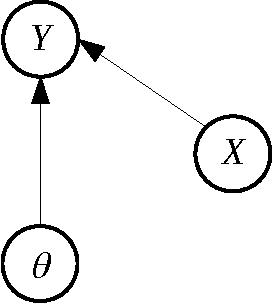
\includegraphics[width=.25\textwidth]{generative.pdf}\label{fig:generative}}
\hspace*{.2\textwidth}
\subfigure[Discriminative model]{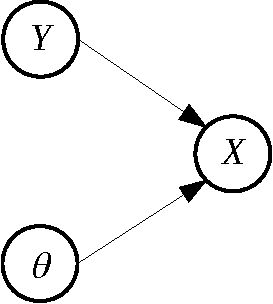
\includegraphics[width=.25\textwidth]{discriminative.pdf}\label{fig:discriminative}}
\caption{Bayesian networks representing generative and discriminative models, where $X$, $Y$ and $\theta$ respectively denote the variable of interest, the data, and the model parameters. Note the marginal independence of~$Y$ and~$\theta$ in the discriminative model.}
\label{fig:graph_comparison}
\end{center}
\end{figure}

Composite likelihood (CL, see \cite{Varin-11} and the references therein) is a semi-generative approach to statistical inference that extends the familiar notion of likelihood without requiring a full generative model. The key idea is to model an arbitrary set of low-dimensional features separately and then combine them, instead of modeling the data distribution as a whole. This may be viewed as a {\em divide and conquer} method to approximate the true but intractable likelihood. While maximum CL does not inherit the general property of maximum likelihood to yield an asymptotically minimum-variance estimator, it is consistent under mild conditions \cite{Xu-11} and may offer an excellent trade-off between computational and statistical efficiency in practice. 

In this note, CL is interpreted as a probabilistic opinion pool of ``agents'' making use of different pieces of information, or clues, extracted from the input data. Each agent acts as an isolated generative model-based statistician and expresses an opinion based on a single clue in the form of a likelihood function of the hidden variables. The agent opinions are then aggregated into a probability distribution on the hidden variables analogous to a Bayesian posterior.

We further argue that a particular log-linear opinion pool yields the best possible predictive distribution in the sense of maximum relative conditional entropy. This perspective entails a method to optimize the weights of the different agents from training data as in a typical discriminative learning scenario. 

%Something for true statisticians. Maybe we could clarify that we use the term ``Bayesian'' in the sense of ``empirical Bayesian'', implying that the parameters $\theta$ are to be estimated somehow contrary to a ``full Bayesian'' approach where they would be integrated out at inference time.


\section{Composite likelihood as opinion pooling}
\label{sec:pool}

Let $Y$ an observable multivariate random variable with sampling distribution $p(y|x)$ conditional on some unobserved variable of interest, $X\in{\cal X}$, where ${\cal X}$ is a known set. Given an experimental outcome $y$, the likelihood is the sampling distribution evaluated at $y$, seen as a function of $x$:
$$
L(x) = p(y|x)
.
$$

This requires a plausible generative model which, for complex data, may be out of reach or involve too many parameters to be estimated. A natural workaround known as {\em data reduction} is to extract some lower-dimensional representation $z=f(y)$, where $f$ is a many-to-one mapping, and consider the potentially more convenient likelihood function:
$$
\ell(x) = p(z|x)
.
$$

Substituting $L(x)$ with $\ell(x)$ boils down to restricting the sample space, thereby  ``delegating'' statistical inference to an ``agent'' provided with partial information. While it is valid for such an agent observing~$z$ only to consider $\ell(x)$ as the likelihood function of the problem, the drawback is that $\ell(x)$ might yield too vague a prediction of~$X$ due to the information loss incurred by data reduction. To make the trick statistically more efficient, we may extract several features, $z_i=f_i(y)$ for $i=1,2,\ldots,n$, and try to combine the likelihood functions $\ell_i(x) = p(z_i|x)$ that they elicit.

If we see the likelihoods as posterior distributions corresponding to uniform priors, this is a classical problem of probabilistic opinion aggregation from possibly redundant sources, for which several methods exist in the literature \cite{Tarantola-82,Genest-86,Garg-04,Allard-12}. We will show in Section~\ref{sec:maxent} that one that is particularly well-suited to our case is the {\em log-linear opinion pool}: 
\begin{equation}
\label{eq:log_pool}
p_\lambda(x|y) = \frac{1}{z_\lambda(y)} \pi(x) \prod_{i=1}^n p(z_i|x)^{\lambda_i},
\end{equation} 
where $\pi(x)$ is some reference distribution or prior, and $\lambda=(\lambda_1,\ldots,\lambda_n)$ is a vector of weights so that the normalizing factor:
$$
z_\lambda(y) = \int \pi(x) \prod_{i=1}^n p(z_i|x)^{\lambda_i} dx
$$
is finite, which holds whenever $\lambda\succeq 0$, {\em i.e.} all weights are positive, assuming that the agent opinions are always upper bounded. Negative weights should be ruled out as the existence condition $z_\lambda(y)<\infty$ would then depend on the particular opinions expressed by the agents. Also note that, while it is possible to have the weights depend on~$y$, there is a strong rational for constant weights as we shall see in the sequel. 

%Strictly positive weights guarantee the so-called 0/1 forcing property, that is, if an hypothesis~$x$ has zero likelihood according to at least one agent, then its consensus probability vanishes too.

% Not clear yet as to what a negative weight could mean!

The log-linear pool~(\ref{eq:log_pool}) bears a striking similarity to Bayes rule, yielding the form: $p_\lambda(x|y)\propto \pi(x) L^c_\lambda(x)$, where the quantity:
\begin{equation}
\label{eq:comp_lik}
L^c_\lambda(x) \equiv \prod_{i=1}^n \ell_i (x)^{\lambda_i}
\end{equation} 
plays the same role as a traditional likelihood function. This expression happens to be known in statistics as a {\em marginal composite likelihood} \cite{Varin-11}. See Appendix~\ref{sec:conditional} for the slightly more general form called {\em conditional composite likelihood}, which can be derived in the same way.

From~(\ref{eq:comp_lik}), we see that CL shares a convenient factorized form with the likelihood derived under the assumption of mutual feature independence, usually referred to as {\em na\"ive Bayes} or {\em simple Bayes} in the machine learning literature, which corresponds to the special case of unitary weights, $\lambda_1=\ldots=\lambda_n= 1$. The clear computational advantage of CL over the true likelihood is that it only requires to evaluate the marginal feature distributions rather than the joint distribution of all features.


\section{Tuning composite likelihood weights}

When the features can be considered exchangeable, it is natural to choose uniform CL weights. The CL is then a scaled version of the na\"ive Bayes likelihood, the common weight value being irrelevant to the maximum CL estimator (MCLE). The weight may be tuned so as to best adjust the pseudo posterior variance matrix to the asymptotic variance matrix of the MCLE \cite{Pauli-11}, or via a close-in-spirit curvature adjustment \cite{Ribatet-12}, in attempts to match the frequentist and composite Bayesian notions of uncertainty.

Ignoring such a goal, another frequent recommandation for CL weights is to sum up to one. This can be motivated in various ways. It turns out that the only pooling operator that does not explicitly depend on~$x$ and preserves {\em external Bayesianity} is the log-linear opinion pool with unit sum weights \cite{Genest-86b}. External Bayesianity essentially means that it should not matter whether the prior is incorporated before or after pooling, provided that all agents agree on the same prior. Another appealing property of log-linear pooling with unit sum weights is to minimize the average Kullback-Leibler (KL) divergence to the agent opinions \cite{Garg-04}. A maximum relative entropy property is also given in \cite{Wang-14}, Theorem~3.

Unit sum weights, however, correspond to the extreme situation where the features are assumed to be maximally redundant, but is clearly ineffective for independent or weakly correlated features, which require weights close to one for the CL to closely approximate the true likelihood. In this case, the CL may be much flatter than it should, leading to severly overestimated credibility sets.

{\color{red} Why is it important to fine-tune the weights?}
We therefore need a method to tune weights that can automatically adjust to the level of statistical dependence beween features.

%Instead, redundancy between agents is assumed by default, and is effectively encoded by the unit sum constraint on weights\footnote{Nevertheless, features which are {\em known} to be mutually independent can be merged into a single feature. This results in increasing their weights in the log-linear pool.}.

\section{Maxent composite likelihood}
\label{sec:maxent}

We can derive composite likelihood from the conditional maximum entropy principle \cite{BergerA-96}. It comes with a method of tuning weights, hence a particular composite likelihood function that we call maxent composite likelihood (MCL).

A cheap MaxEnt argument was already given by \cite{Wang-14}  (standard, non-conditional MaxEnt at fixed $y$, hence just an existence result but no feasible weight tuning).

What we do here is maximum {\em conditional} entropy. It's slightly more complex than a simple $I$-projection. The search space is a set of predictive distributions compatible with mean log-likelihood contraints. If I know the generative distribution, I know the expected log-likelihood.

We work with inequality constraints to force $\lambda\geq 0$:
$$
E[\log p(z_i|x)] \geq c_i \equiv \int \pi(x)p(z_i|x) \log p(z_i|x) dx dy
$$

What does the constraint mean? It means that a model is admissible if it compresses the data at least as well as all my agents. So we are not assuming that the generative models are {\em true}. We only assume that they are useful to compress the (reduced) data. Connection to MDL. 

Why not using the feature-based posteriors or Bayes factors rather than the likelihoods? It's a possibility (perhaps a connection here with Gr\"unwald's luckiness). A justification for not doing it is that the coordinator should discard the priors used by the agents. The constraints are not purely evidence-based since the moments depend on the coordinator's prior but it is arguable a mess of priors wouldn't be good.

Intuition behind weights: Lagrange multipliers to enforce a constraint... Notion of feature relevance. But does $\lambda_1>\lambda_2$ imply that $z_1$ is more relevant than $z_2$? 

The derivation assumed the marginal distribution of the data $h(y)$ to be known. In practice, it is estimated by the empirical distribution just like the moments are estimated.

Game theoretic interpretation \cite{Grunwald-04}.

The dual function boils down to the famous cross-entropy.

Single feature case ($y=z$): the maxent solution has the form $p(x|y)\propto\pi(x)p(y|x)^\lambda$. We expect to have $\lambda=1$ but it's not necessarily the case. It is if $h(y)=\int\pi(x)p(y|x)dx$ because then $h(y)p(x|y)=\pi(x)p(y|x)$ so the constraint is verified (and active). This also tells us that the data marginal should be consistent with the prior on labels for this much expected consistency property to hold. So, either weight datapoints so as to match a desired prior (e.g., uniform) or take the empirical distribution of labels as the ``prior''. 

Which brings another question: in this case, the (unique) weight is insensitive to the prior -- is it true in general? The answer is no. The weights generally depend on the prior. Hence the maxent composite likelihood is prior-dependent. This is an important conceptual difference with the classical notion of likelihood.

\section{Super composite likelihood}
\label{sec:super}

When chosen for computational simplicity, clues may not only convey limited information at individual level: their informativeness may also be very much hypothesis-dependent. Consider, for instance, diagnosing a disease from a routine medical checkup. Body temperature may point to a bacterial infection by comparison with normality, but would not help detecting a non-infectious cardiovascular disease -- and conversely for, say, blood pressure.

This motivates a more general setting where clues can be weighted differently depending on hypotheses.

What happens if we use mean-values constraints conditional on $x$ instead of jointly averaged over $x$ and $y$? This boils down to picking functions of the form:
$$
\chi(x-a)\ell_i(x,y)
$$

The answer is that the maxent solution has the form:
$$
p_\lambda(x|y) = \pi(x) \prod_i p(z_i|x)^{\lambda_i(x)}
$$

In other words, the weights become dependent on the variable of interest. This is the super composite likelihood idea.


\section{Composite EM algorithm for unsupervised learning}
\label{sec:gem}

In a nutshell: alternate unsupervised learning of partial model parameters ($M$-step) and re-estimation of label posteriors via maxent ($E$-step). 

$M$-step: given a posterior estimate $q(x|y)$, do just as if the features were independent and solve: 
$$
\max_\theta
\int \sum_i h(y)q(x|y) \log p_\theta(z_i,x) dx dy
$$

Note we can estimate cross-feature parameters such as class proportions.

Surrogate $E$-step: given generative parameters, recompute the moment constraints and update $q(x|y)$ according to the conditional maxent principle:
$$
\min_q
\int h(y)q(x|y) \log \frac{q(x|y)}{\pi(x)} dx dy
$$
s.t.
$$
\int h(y)q(x|y)\log p_\theta(z_i|x) dx dy \geq \int \pi(x)p_\theta(z_i|x)\log p_\theta(z_i|x) dx dy
$$

However, there is an important issue: how is $h(y)$ defined in both the $M$- and $E$-steps? In supervised context, $h(x,y)$ can be defined beforehand as the prior-corrected empirical distribution:
$$
h(x,y) = \pi(x) \frac{h_0(x,y)}{h_0(x)},
$$
where $h_0(x,y)$ is the raw empirical distribution. In unsupervised context, the best we can do is to replace $h_0(x,y)$ with $h_0(y)q(x|y)$, implying that the empirical distribution of $y$ is reweighted according to:
$$
h(y) = \sum_i w_i\delta(y-y_i),
\qquad
w_i = \int \pi(x)\frac{q(x|y_i)}{\sum_j q(x|y_j)} dx,
$$
which needs to be done each time $q(x|y)$ is updated, that is, after each $E$-step.

The other option is to keep $h(y)$ constant throughout the iterations but adapt $\pi(x)$ as the marginal distribution of labels learned in the $M$-step. In this case, it's no longer a ``prior''. 

Are we minimizing a unique functional as in the variational EM algorithm? Possibly not. We may see this generalization as a two-player game. One player tries to predict several data features independently. The other player tries to predict labels. Together, they find patterns (clusters) in unlabeled data. Does the more general version converge? Does the game have a value? And so on.

In the case of a single feature, is this the well-known EM? The $M$-step is clearly the same, what about the $E$-step? It is the same if $h(y)p_\theta(x|y)=p_\theta(y|x)\pi(x)$. However, this condition won't hold if $h(y)$ is an empirical distribution... In this special case, the ``E player'' could use the data distribution model produced by the ``M player'' instead of the empirical one but, more generally, there is no data distribution model so he has to stick to the empirical one.

The maxent is a surrogate for the $E$-step. It reflects the lack of a full model $p_\theta(x,y)$.

% Accounting here for Xi'An comment on xianblog.wordpress.com
% The sum of the powers is constrained to be equal to one, even though
% I do not understand why the dimensions of the projections play nog
% role in this constraint. Simplicity is advanced as an argument,
% which sounds rather weak…
%This simple constraint is implied by the external Bayesianity requirement: as it turns out, the only aggregation operator which is both externally Bayesian and independent from $x$ boils down to plugging a composite likelihood with unit sum weights into Bayes rule, hence extending the classical notion of likelihood in Bayesian analysis.


\section{Discussion}
\label{sec:discussion}

Deep learning is discriminative...

CL is a concept from computational statistics that has mainly been developed so far in a frequentist perspective as a surrogate for the maximum likelihood method. We have shown a deep connection between CL and probabilistic inference, thereby establishing CL as a class of discriminative models. Because CL is built from a set of marginal feature-specific generative distributions, it is in essence a two-step semi-generative, semi-discriminative learning approach. In the first, ``generative'' phase, the feature distributions are learned; in the second, ``discriminative'' phase, the feature weights are learned. This strategy can be thought of as a form of non-adaptive boosting.

%The first phase corresponds to the training of ``weak learners''. The second phase amounts to a form of boosting. 

A purely discriminative learning could be used instead but...
Why potentially more efficient than pure discriminative training: because generative training is always more efficient than discriminative training if models are comparable. So the key point is that ``we have less parameters in the discriminant phase". Good in small datasets. But also in asymptotic regime if the features are weakly or highly correlated (???).

Logistic regression / naive Bayes example. Under homoscedasticity (assuming that each feature has class-independent variance), CBI is equivalent to logistic regression -- because the predictive distribution family is the same. This is a case where BCI brings nothing. But consider heteroscedasticity, then BCI yields a quadratic classifier. Compared to a fully discriminative model, the number of parameters to learned in the discriminative phase is reduced by half.

The first training phase is easier if supervised but could be unsupervised too (using mixture models). How do we then deal with label switching issues? Can we safely assume conditional feature independence {\em in the generative training phase}? I believe so provided that the marginal distribution parameters are disjoint. It's obvious in the supervised learning scenario.

If unsupervised, the first learning phase could be compared with contrastive pre-training of RBMs \cite{Hinton-06,Fischer-14}, which also optimize parameters for generation of observable features. BCI is comparable with an RBM with a single output unit (which is just a generative model assuming conditionial feature independence). The key difference is that the RBM is a full generative model while BCI only deals with marginal models, hence relying on weaker assumptions. This won't change anything in the pre-training phase but RBMs have to deal with more parameters in the generative learning phase. In fully supervised context, RBM pre-training is pointless since all parameters learned in the first phase will be overwritten. In BCI, pre-training is crucial even in supervised context because the parameters learned in the discriminative phase (the feature weighs) describe a sub-manifold of the predictive distribution family.

Needs features. Not a representation learning method, but could be coupled why not.


%{\color{red} Moreover, while RBM parameters are typically refined in a supervised discriminative learning step, disjoint set of parameters for SCL. Dunno how to say that.} 

%In such context, SCL competes with classical discriminative models (logistic regression, Gaussian processes \cite{Rasmussen-06}, maximum entropy models \cite{BergerA-96}, etc.), and may compare more or less favorably in practice depending on the amount of training data. For relatively small training datasets, we may hope for more accurate inference using~SCL than using traditional discriminative models, extrapolating from the results of \cite{Ng-01} regarding the comparison between logistic regression and na\"ive Bayes classifiers.
%{\color{red}Ici, il manque la comparaison avec les RBMs qui ne sont pas (forcement) des modeles discriminatifs.}

%%, hence alleviating the need for heavily supervised model training

%In summary, CL has the potential to yield weakly supervised or unsupervised Bayesian-like inference procedures depending on the particular task at hand. This property reflects the encoding of statistical relationships between the data and {\em all} unknown parameters. CL thus appears as a trade-off between generative models, which are optimal for unsupervised learning but possibly intractable, and traditional discriminative models (logistic regression, Gaussian processes \cite{Rasmussen-06}, maximum entropy models \cite{BergerA-96}, etc.), which are inherently supervised. CL models are discriminative models assembled from atomic generative models and, from this point of view, may be considered as {\em semi-generative} models.

%CL may be considered as a {\em semi-generative} model: a discriminative model assembled from partial generative models.

%As a note of caution, we shall stress that the pre-determined weights assigned to the different associations between observed and unobserved values represent prior knowledge regarding the informativeness of clues. A poor choice of weights will inevitably result in a poor approximation to the ``true'' Bayesian posterior -- the posterior that would be obtained from a realistic generative model if it was tractable. In future work, we will investigate feature selection strategies to mitigate this problem.

% Improve the discussion on following aspects:
% ** Why is it compatible with unsupervised learning? Give more insight.
% ** Stress the contribution: class-specific weighting.
% * Pivotality argument.
% * Bayes is a special case of composite Bayes.

{\color{red}Product of fucking experts \cite{Hinton-02}. Log-linear pool to build a generative model (assuming in fact independence between experts). Better seen as a ``log-mixture model''. Sounds like each expert is associated with a class, so it's the same as a RBM. Contrastive learning approximates ML parameter estimation. The experts are learning jointly. It's just a generative model.}

{\color{red}Two-step training: generative phase then discriminative phase. Why is it cool?}

{\color{red}CBI is just a way to reweight Naive Bayes. What's the big deal? Can we really expect massively superior performance? Are we just talking about realistic credibility sets?}


\appendix

\section{Conditional composite likelihood}
\label{sec:conditional}

As a straightforward  extension of marginal CL, each feature-based likelihood may be conditioned by an additional ``independent'' feature $z^c_i = f^c_i(y)$ considered as a predictor of the ``dependent'' feature, $z_i=f_i(y)$, yielding the more general form:
\begin{equation}
\label{eq:cond_feat_lik}
\ell_i(x) = p(z_i|x,z^c_i).
\end{equation}

Conditioning may be useful if it is believed that $z^c_i$ alone is little or not informative about $x$, but can provide relevant information when considered jointly with $x$, as in the case of regression covariates, for instance. Equation~(\ref{eq:comp_lik}) then amounts to conditional CL \cite{Varin-11}, a more general form of CL also including Besag's historical {\em pseudo-likelihood} \cite{Besag-74} developed for image segmentation.


\section{Minimally discriminative model}

Let $\pi(x)$ some reference distribution that represents full
uncertainty about $X$. We wish to select the joint distribution
$p(x,y)$ that minimizes:
$$
I(p) = \int p(x,y) \log \frac{p(x|y)}{\pi(x)} dy,
$$ subject to feature mean-value constraints of the form:
$$
\int p(x,y) f(x,y) dx dy = \mu.
$$

There are two special cases of this problem in the literature.  On the
one hand, the {\em maximum entropy classifier} \cite{BergerA-96}
incorporates the constraint that $p(y)$ be known, however we will see
that this is not necessary. The {\em minimally informative likelihood}
method \cite{Yuan-99b,Yuan-99}, on the other hand, imposes that
$p(x)=\pi(x)$, hence assuming the form $p(x,y)=\pi(x)p(y|x)$. We won't
make such assumptions here and will consider the case where $\mu$ is
completely unknown.

The above problem is seen to be equivalent to minimizing the auxiliary
objective function:
$$
I(p,m) 
= \int p(x,y) \log \frac{p(x,y)}{\pi(x)m(y)} dxdy,
$$ over $p$ and $m$, subject to the same constraints on $p$. We note
that $I(p,m)=I(p)+D(p_y\|m)$, showing that the auxiliary function
essentially adds a penalty term to the actual objective in order to
force $p(y)$ close to $m(y)$.

Minimizing $I(p,m)$ along both $p$ and $m$ is basically a minimum KL
divergence problem between two convex distribution spaces, so there
must be a unique solution {\bf -- to be checked in
  \cite{Cover-91}}. It is similar to the rate-distortion problem in
information theory, which may be solved by alternate minimization,
yielding a Blahut-Arimoto algorithm.
\begin{itemize}
\item {\em Let's call it A-step}. Optimize $p(x,y)$ at fixed $m$
  s.t. constraint:
$$
\exists \lambda, \qquad
p_{\lambda,m}(x,y) = \frac{1}{Z(\lambda, m)} \pi(x) m(y) e^{-\lambda^\top t(x,y)}
$$
The actual $\lambda$ is found my maximizing the dual function
$\psi(\lambda,m)$, see below.
\item {\em Let's call it B-step}. Optimize $m(y)$ at fixed $p(x,y)$:
$$
m(y) = \int p(x,y) dx
$$
\end{itemize}

Upon convergence, the algorithm outputs both joint and marginal
distributions $p_{\star}(x,y)$ and $m_{\star}(y)$ that both depend on
$\mu$. By construction, we have that $p_{\star}(y) = m_{\star}(y)$,
therefore $p_\star(x|y)=p_{\star}(x,y)/m_{\star}(y)$.


\section{Comparison with maximum entropy classifier}

Lagrangian...
$$
{\cal L}(p,m,\lambda)
= 
\int p(x,y) \log \frac{p(x,y)}{\pi(x)m(y)} dxdy
+
\lambda^\top \left( 
\int p(x,y) f(x,y) dydy - \mu 
\right)
$$ where $\lambda$ represents a vector-valued Lagrange multiplier. At
fixed $m$, the solution has the form:
$$
p_{\lambda,m}(x,y) = \frac{1}{Z(\lambda,m)}
\pi(x) m(y) e^{-\lambda^\top f(x,y)} 
$$

Note that this implies that the conditional distribution is
independent of $m$ once $\lambda$ is determined,
$$
p_\lambda(x|y) = \frac{1}{z(\lambda,y)} \pi(x) e^{-\lambda^\top f(x,y)} 
$$

Also, the marginal is a modulation of $m(y)$:
$$
p_{\lambda,m}(y) = \frac{z(\lambda,y)}{Z(\lambda,m)} m(y)
$$

Dual function at fixed $m$:
$$
\psi(\lambda,m) 
\equiv \min_p {\cal L}(p,m,\lambda)
= 
- \log Z(\lambda,m) - \lambda^\top \mu
.
$$ 

An alternative expression is:
$$
\psi(\lambda, m)
= 
\int h(x,y) 
\log \frac{p_{\lambda,m}(x,y)}{\pi(x)m(y)} dxdy,
$$ where $h(x,y)$ is any distribution statisfying the
constraints. This shows that maximizing the dual function at fixed $m$
is essentially the same as minimizing the KL divergence
$D(h\|p_{\lambda,m})$ over $\lambda$, in other words fitting $h(x,y)$
by some distribution of the form $p_{\lambda,m}$. The fact that the
result does not depend on the particular $h(x,y)$ that is chosen, as
long as it satifies the constraint, is a general property of
exponential families.

We also have that the dual function associated with $I(p)$ reads:
\begin{eqnarray*}
\psi(\lambda) 
 & = & \min_m \psi(\lambda, m)\\
 & = & \int h(x,y) \log \frac{p_{\lambda}(x|y)}{\pi(x)} dxdy\\
 & = & -\int h(y) \log z(\lambda,y) dy - \lambda^\top \mu
\end{eqnarray*}

But, wait, that's exactly what we get in the maximum entropy
classifier! So, at the end of the day, we simply got an alternative
method to learn $\lambda$ in the maximum entropy classifier, i.e. the
Blahut-Arimoto algorithm as opposed to a brute-force maximization of
$\psi(\lambda)$. Both methods will converge to the same $\lambda$...

What it essentially means is that the optimal $\lambda$ is insensitive
to $m(y)$ as long as $m(y)$ is compliant in the sense that:
$$
m(y) = \int h(x,y) dx,
$$ for some distribution $h(x,y)$ statisfying the constraint. This is
true for the optimal $m_\star(y)$ output by the BA algorithm, but
also, for instance, for the empirical distribution of observations in
a training dataset used to estimate $\mu$, as proposed in
\cite{BergerA-96}. The only special property of $m_\star(y)$ is to
yield the full Bayesian model $p_\star(x,y)=p_\star(x|y)m_\star(y)$
that minimizes the discrimination information. We may not care too
much about that in practice since we will only use $p_\star(x|y)$. 

\section{Comparison with minimally informative likelihood}

Yuan \cite{Yuan-99} considered the situation where we add the
constraint that $p(x)=\pi(x)$ to the minimum discrimination inference
problem. Unknown is then the conditional distribution
$p(y|x)$. Lagrangian...
\begin{eqnarray*}
{\cal L}(p,m,\lambda)
 & = & 
\int \pi(x)p(y|x) \log \frac{p(y|x)}{m(y)} dxdy
+
\lambda^\top \left( 
\int \pi(x)p(y|x) f(x,y) dydy - \mu 
\right) \\
 & = & 
\int \pi(x)
\left( 
\int
p(y|x) \log \frac{p(y|x)}{m(y)} dy
+
\lambda^\top 
\int p(y|x) f(x,y) dy
- \mu 
\right)
dx 
\end{eqnarray*}

The derivative is given by,
$$
\frac{\partial\cal L}{\partial p(y|x)}
= 
\pi(x)\left[ 
1 + \log \frac{p(y|x)}{m(y)} 
+ \lambda^\top f(x,y)
\right],
$$
hence the optimal model at fixed $m$ has the form:
$$
p_{\lambda,m}(y|x) = \frac{1}{Z(\lambda,m,x)} m(y) e^{-\lambda^\top f(x,y)} 
$$

Note that the induced posterior distribution $p_{\lambda,m}(x|y)$ has
a different form from above unless the normalizing factor
$Z(\lambda,m,x)$ turns out independent from $x$. If this is not the
case, we no longer have the property that $p_{\lambda,m}(x|y)$ is
independent from $m$ given $\lambda$.

Dual function...
$$
\psi(\lambda,m) 
=
- \int \pi(x) \log Z(\lambda, m, x) dx
- \lambda^\top \mu
$$

Equivalently, for any distribution under the form $\pi(x)h(y|x)$ that
satisfies the moment constraint, we have:
$$
\psi(\lambda,m) 
=
\int \pi(x) h(y|x) \log \frac{p_{\lambda,m}(y|x)}{m(y)} dxdy
$$

Now, the real question is why should we constrain $p(x)$, which boils
down to a Bayesian prior in this context, to be the same as our
reference $\pi(x)$? It only makes sense if we want our inference to
stick to a generative modeling paradigm... but haven't we already
given up on that? Therefore, unless we find a good reason not to, we
won't impose the $p(x)=\pi(x)$ constraint, thereby allowing for a
discrepancy between the reference and the prior.


\section{Discriminative vs. semi-discriminative}

Let's go back to the equivalence we found between our approach and the
maximum entropy classifier (MCE) \cite{BergerA-96}. We have said that
the former is essentially a re-formulation of MCE.

But the re-formulation also conveys a generalization of MCE if,
instead of letting $m$ being an arbitrary distribution, we restrict
its search space to some set of acceptable reference
distributions. Would such a strategy be useful? 

Recall that the method selects the joint distribution that minimizes
discriminative information, as defined by $I(p)$:
$$
I(p) 
= \int p(x,y)\log\frac{p(x|y)}{\pi(x)} dxdy
= E_Y[D(p_{x|y}\|\pi)]
$$

The latter characterization reminds us that discriminative information
is defined in an average sense. The corresponding posterior $p(x|y)$
may not be conservative for some $y$, in particular those that are
unlikely under $p(y)$. It would be a problem if that's the case for
the particular data at hand. For that to happen rarely, the ideal
$p(y)$ would be the ``true'' marginal distribution of $Y$.

However, for vague mean value constraints, nothing may prevent the
optimal $m_\star(y)$ from departing significantly from that ideal
distribution. In fact, we can show that $m_\star(y)$ only has mass at
$y$ values that maximize $z(\lambda_\star,y)$, and is therefore likely
sparse. This is because $m_\star$ minimizes $\psi(\lambda_\star,m)$,
which is equivalent to maximizing $Z(\lambda_\star,m)$ and we have:
$$
Z(\lambda, m) = \int m(y) z(\lambda, y) dy.
$$

In other words, the solution to our problem may be singular! It does
not hurt since, as discussed above, one may alternatively fix $m(y)$
to some pre-defined distribution... but this, in practice, restricts
the method to supervised learning situations.

We may not face this issue with the MIL method, which further imposes
the prior on $X$, so all the information from the constraints goes
into specifying a possibly reasonable generative model.



\bibliographystyle{abbrv}
\bibliography{cvis,stat,alexis}

%%\input{draft.biblio}

\end{document}


\end{document}


\end{document}


\end{document}
